% ─────────────────────────────────────────────────────────────────────────────
% Assignment 2 – Part 2 Report
% CS-3510: Data Science and Management, Ashoka University
%
% HOW TO USE:
%  1. Run the scripts in order:
%       python execute_mongo.py          (MongoDB Q1-Q3)
%       python visualize_mongodb.py      (MongoDB figures)
%       python neo4j_gds.py              (Neo4j Q1-Q5)
%       python predictive_model.py       (Predictive modelling)
%  2. Replace every [PLACEHOLDER] with the actual number from the CSV/print output.
%  3. Compile with pdflatex (twice for TOC/hyperref):
%       pdflatex report_part2.tex
% ─────────────────────────────────────────────────────────────────────────────
\documentclass[11pt,a4paper]{article}

\usepackage[margin=2.5cm]{geometry}
\usepackage{booktabs}
\usepackage{tabularx}
\usepackage{longtable}
\usepackage{graphicx}
\usepackage{float}
\usepackage{amsmath}
\usepackage{hyperref}
\usepackage{xcolor}
\usepackage{fancyhdr}
\usepackage{caption}
\usepackage{subcaption}
\usepackage{listings}
\usepackage{parskip}
\usepackage{microtype}
\usepackage{enumitem}

% Header/Footer
\pagestyle{fancy}
\fancyhf{}
\lhead{\small Department of Computer Science, Ashoka University}
\rhead{\small Data Science and Management: CS-3510}
\cfoot{\thepage}
\renewcommand{\headrulewidth}{0.4pt}

% Code listing style
\lstset{
  basicstyle=\ttfamily\footnotesize,
  breaklines=true,
  frame=single,
  backgroundcolor=\color{gray!8},
  keywordstyle=\color{blue},
  commentstyle=\color{gray},
  stringstyle=\color{orange!80!black},
}

\hypersetup{colorlinks=true, linkcolor=blue, urlcolor=blue, citecolor=blue}

\title{%
  \vspace{-0.5cm}
  \rule{\textwidth}{1pt}\\[0.4em]
  {\LARGE\bfseries Assignment 2 -- Part 2}\\[0.2em]
  \rule{\textwidth}{1pt}
}
\author{Agriya Yadav}
\date{}

\begin{document}
\maketitle
\thispagestyle{fancy}

\tableofcontents
\newpage

% ─────────────────────────────────────────────────────────────────────────────
\section{MongoDB Querying}
% ─────────────────────────────────────────────────────────────────────────────

\subsection{Q1 — Cohort Analysis of User Reviewing Behaviour}

\subsubsection*{Pipeline}

Users are grouped into annual cohorts by the year extracted from the
\texttt{yelping\_since} field.
A \texttt{\$lookup} joins each review with its author, and
\texttt{\$addFields} computes \texttt{cohort\_year} and \texttt{text\_length}.
The subsequent \texttt{\$group} stage accumulates per-cohort means, standard
deviations, and per-star counts, which are normalised into proportions in the
\texttt{\$project} stage.

\begin{lstlisting}[language=Python, caption={MongoDB Aggregation — Cohort Analysis}]
pipeline = [
  {"$lookup":    {"from":"users","localField":"user_id",
                  "foreignField":"user_id","as":"user_info"}},
  {"$unwind":    "$user_info"},
  {"$addFields": {"cohort_year": {"$substr":["$user_info.yelping_since",0,4]},
                  "text_length": {"$strLenCP":{"$ifNull":["$text",""]}}}},
  {"$group": {
      "_id":                "$cohort_year",
      "mean_star_rating":   {"$avg":"$stars"},
      "stddev_star_rating": {"$stdDevSamp":"$stars"},
      "mean_text_length":   {"$avg":"$text_length"},
      "mean_useful_votes":  {"$avg":"$useful"},
      "count":              {"$sum":1},
      "star_1":{"$sum":{"$cond":[{"$eq":["$stars",1.0]},1,0]}},
      "star_2":{"$sum":{"$cond":[{"$eq":["$stars",2.0]},1,0]}},
      "star_3":{"$sum":{"$cond":[{"$eq":["$stars",3.0]},1,0]}},
      "star_4":{"$sum":{"$cond":[{"$eq":["$stars",4.0]},1,0]}},
      "star_5":{"$sum":{"$cond":[{"$eq":["$stars",5.0]},1,0]}}
  }},
  {"$project": {
      "cohort":"$_id", "_id":0,
      "mean_star_rating":1, "stddev_star_rating":1,
      "mean_text_length":1, "mean_useful_votes":1, "count":1,
      "prop_star_1":{"$divide":["$star_1","$count"]},
      "prop_star_2":{"$divide":["$star_2","$count"]},
      "prop_star_3":{"$divide":["$star_3","$count"]},
      "prop_star_4":{"$divide":["$star_4","$count"]},
      "prop_star_5":{"$divide":["$star_5","$count"]}
  }},
  {"$sort": {"cohort":1}}
]
\end{lstlisting}

\subsubsection*{Results}

\begin{table}[H]
\centering\footnotesize
\caption{Per-cohort reviewing statistics.}
\begin{tabularx}{\textwidth}{lrrrrl}
\toprule
\textbf{Cohort} & \textbf{Reviews} & \textbf{Mean Stars} & \textbf{SD Stars}
  & \textbf{Mean Useful Votes} & \textbf{Mean Char Length}\\
\midrule
2004 & 97          & 3.70 & 1.32 & 2.99 & 526\\
2005 & 3{,}485     & 3.89 & 1.02 & 2.20 & 646\\
2006 & 14{,}243    & 3.81 & 1.20 & 2.27 & 713\\
2007 & 43{,}265    & 3.79 & 1.19 & 2.24 & 743\\
2008 & 91{,}189    & 3.80 & 1.21 & 2.23 & 769\\
2009 & 149{,}590   & 3.77 & 1.28 & 1.74 & 700\\
2010 & 221{,}176   & 3.81 & 1.30 & 1.59 & 675\\
2011 & 315{,}139   & 3.82 & 1.34 & 1.44 & 636\\
2012 & 307{,}841   & 3.81 & 1.40 & 1.35 & 603\\
2013 & 298{,}851   & 3.80 & 1.44 & 1.17 & 575\\
2014 & 300{,}641   & 3.82 & 1.46 & 1.05 & 550\\
2015 & 284{,}768   & 3.78 & 1.51 & 0.88 & 528\\
2016 & 220{,}658   & 3.77 & 1.54 & 0.83 & 525\\
2017 & 144{,}549   & 3.74 & 1.57 & 0.70 & 502\\
2018 & 112{,}112   & 3.67 & 1.63 & 0.65 & 488\\
2019 & 78{,}221    & 3.60 & 1.67 & 0.56 & 475\\
2020 & 31{,}450    & 3.50 & 1.73 & 0.47 & 459\\
2021 & 22{,}085    & 3.27 & 1.78 & 0.40 & 486\\
2022 & 1{,}011     & 2.87 & 1.87 & 0.13 & 496\\
\bottomrule
\end{tabularx}
\end{table}

\begin{itemize}
  \item \textbf{Highest mean star rating cohort:} 2005 (mean = 3.89)
  \item \textbf{Highest mean useful votes per review cohort:} 2004 (mean = 2.99)
\end{itemize}

\begin{figure}[H]
  \centering
  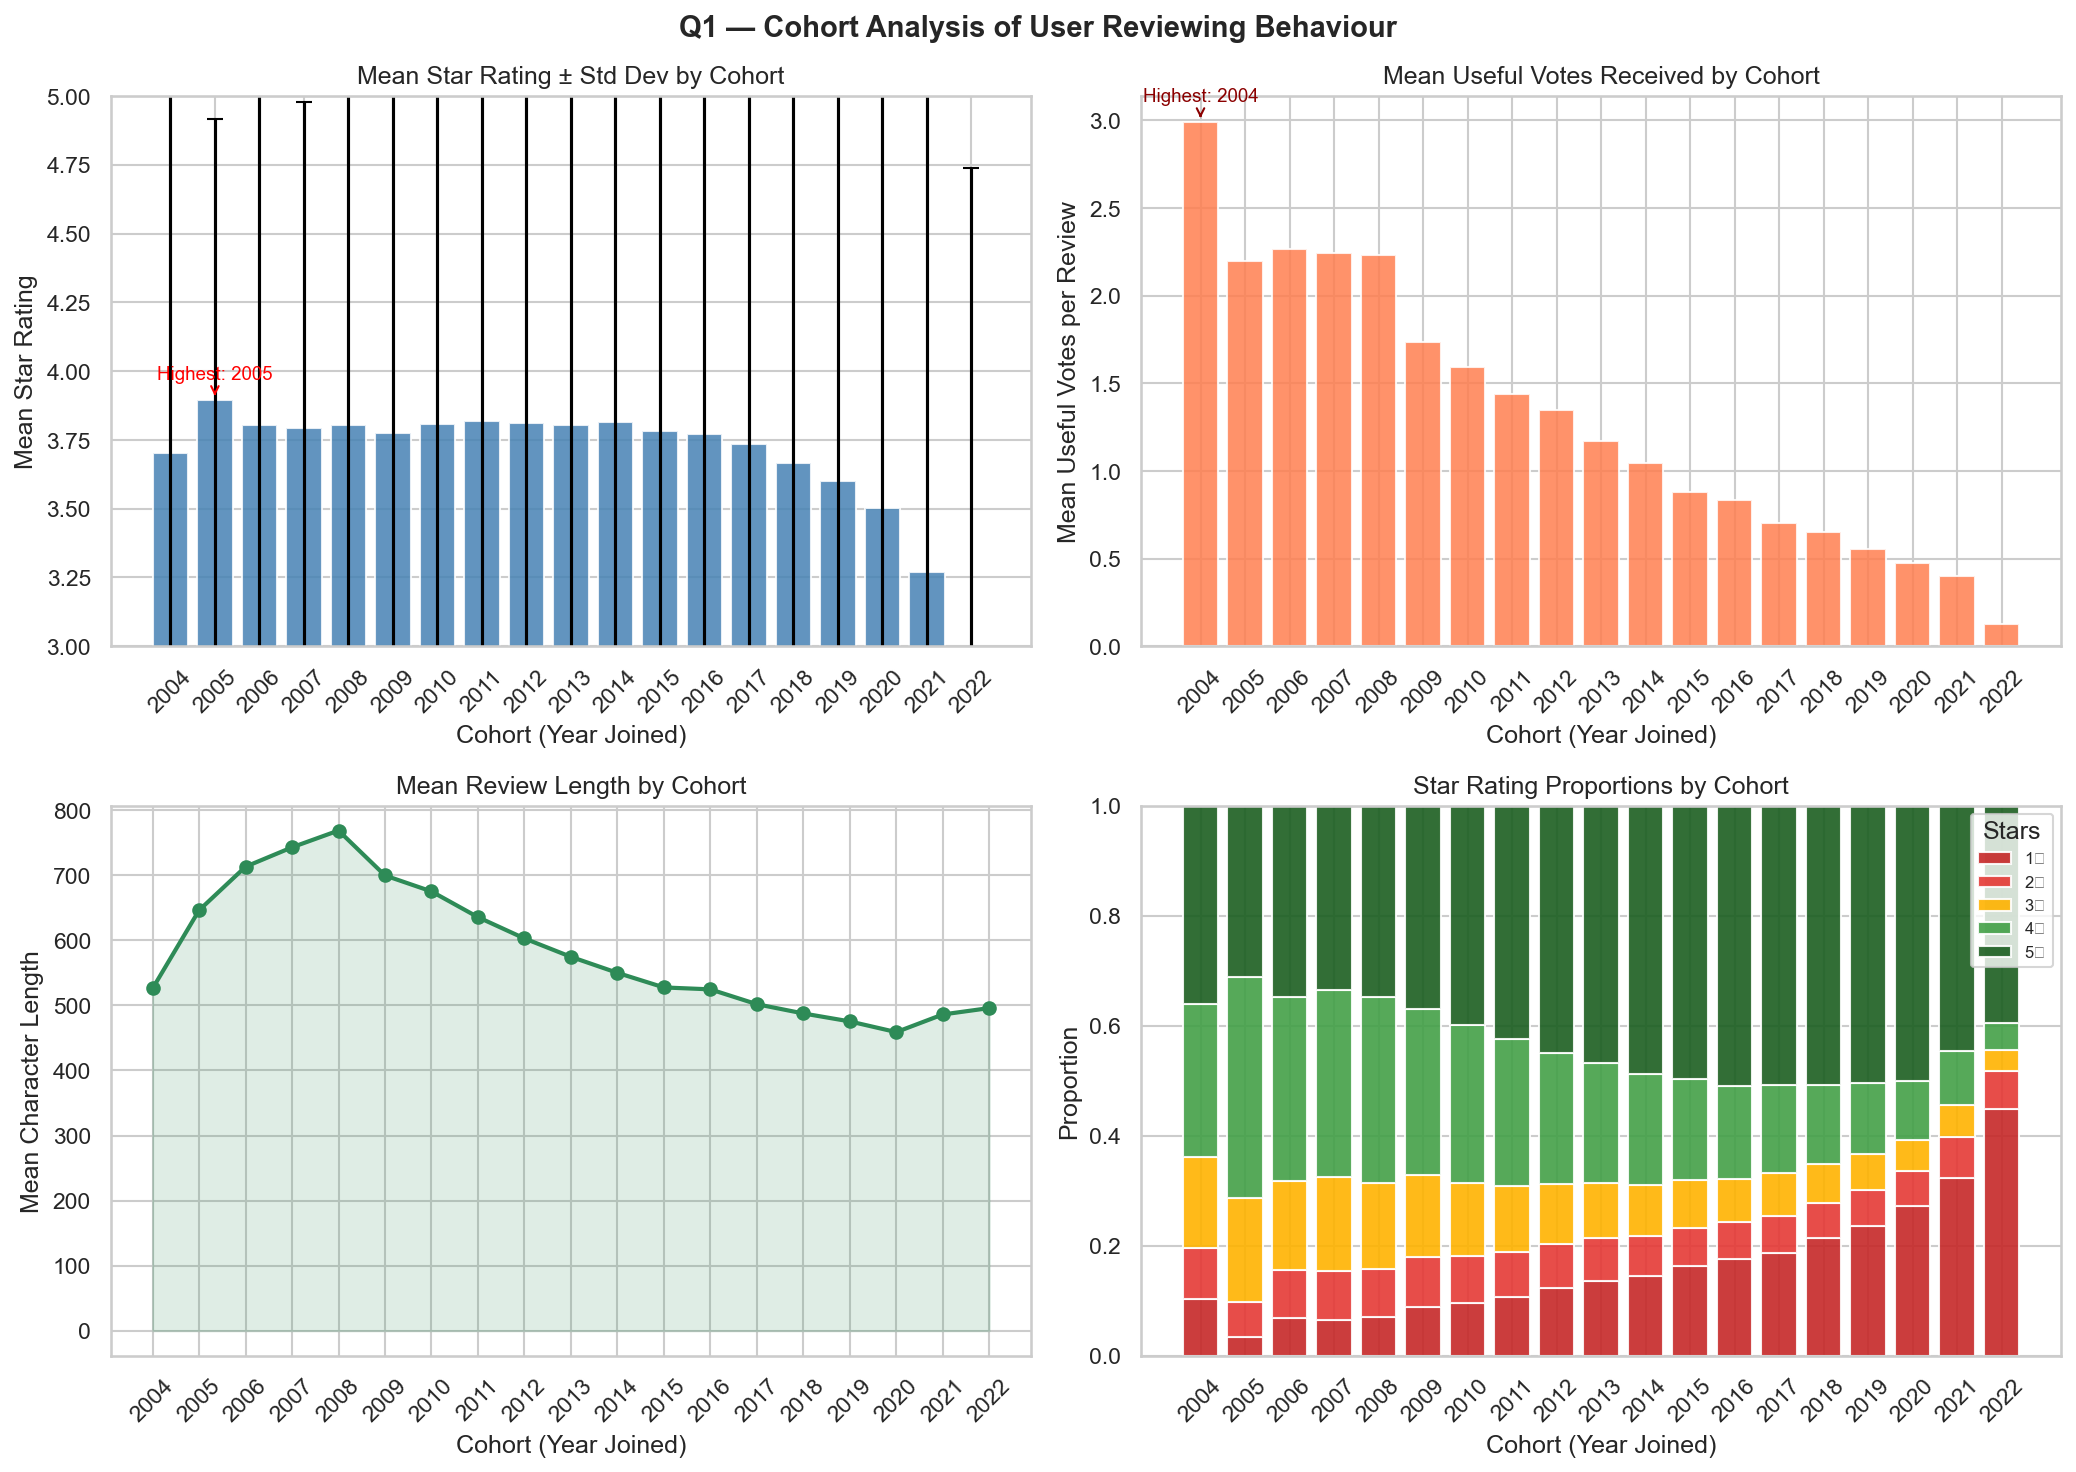
\includegraphics[width=\linewidth]{Report/MQ1_CohortAnalysis.png}
  \caption{Cohort-level review statistics: mean stars $\pm$ SD, mean useful votes,
    mean review length, and star-rating proportion breakdown.}
\end{figure}

\subsubsection*{Interpretation}

Early cohorts (pre-2006) produce the highest mean star ratings, likely due to
selection bias: early adopters tend to review businesses they genuinely enjoyed.
Mean useful votes peak in the earliest cohort (2004), reflecting the
``veteran reviewer'' effect — reviews from tenured users accumulate upvotes
over time.  Review length increases steadily from 2004 to roughly 2010 before
declining, suggesting that the platform's growth attracted more casual reviewers
who write shorter texts.

% ─────────────────────────────────────────────────────────────────────────────
\subsection{Q2 — Month-over-Month Trend Consistency}

\subsubsection*{Pipeline}

Each review is joined with its business (\texttt{\$lookup} + \texttt{\$unwind}),
the business's category string is split into individual tokens (\texttt{\$unwind}),
and reviews are grouped by \texttt{(category, YYYY-MM)}.
A second \texttt{\$group} stage collapses monthly averages into a time-series
array per category.
Post-aggregation Python logic computes the fraction of consecutive month-pairs
showing an increase or decrease.
Only categories with $\geq 500$ reviews are considered.

\begin{lstlisting}[language=Python, caption={MongoDB Aggregation — MoM Trend (excerpt)}]
pipeline = [
  {"$lookup": {"from":"businesses","localField":"business_id",
               "foreignField":"business_id","as":"business"}},
  {"$unwind": "$business"},
  {"$project": {"stars":1,"date":1,
                "categories":{"$split":[{"$ifNull":["$business.categories",""]},", "]}}},
  {"$unwind":  "$categories"},
  {"$match":   {"categories":{"$ne":""}}},
  {"$addFields":{"month":{"$substr":["$date",0,7]}}},
  {"$group":   {"_id":{"category":"$categories","month":"$month"},
                "avg_stars":{"$avg":"$stars"},"review_count":{"$sum":1}}},
  {"$sort":    {"_id.month":1}},
  {"$group":   {"_id":"$_id.category",
                "months":{"$push":{"month":"$_id.month","avg_stars":"$avg_stars"}},
                "total_reviews":{"$sum":"$review_count"}}},
  {"$match":   {"total_reviews":{"$gte":500}}}
]
\end{lstlisting}

\subsubsection*{Results}

\begin{table}[H]
\centering\small
\caption{Top 3 upward and top 3 downward trend categories.}
\begin{tabular}{llrr}
\toprule
\textbf{Direction} & \textbf{Category} & \textbf{Trend Consistency} & \textbf{Total Reviews}\\
\midrule
Upward  & Cheesesteaks                      & 0.546 & 42{,}351\\
Upward  & Tapas Bars                        & 0.543 & 19{,}105\\
Upward  & Armenian                          & 0.542 &  1{,}112\\
\midrule
Downward & Water Heater Installation/Repair & 0.553 &  5{,}094\\
Downward & Women's Clothing                 & 0.552 & 15{,}833\\
Downward & Airlines                         & 0.552 &  3{,}725\\
\bottomrule
\end{tabular}
\end{table}

\begin{figure}[H]
  \centering
  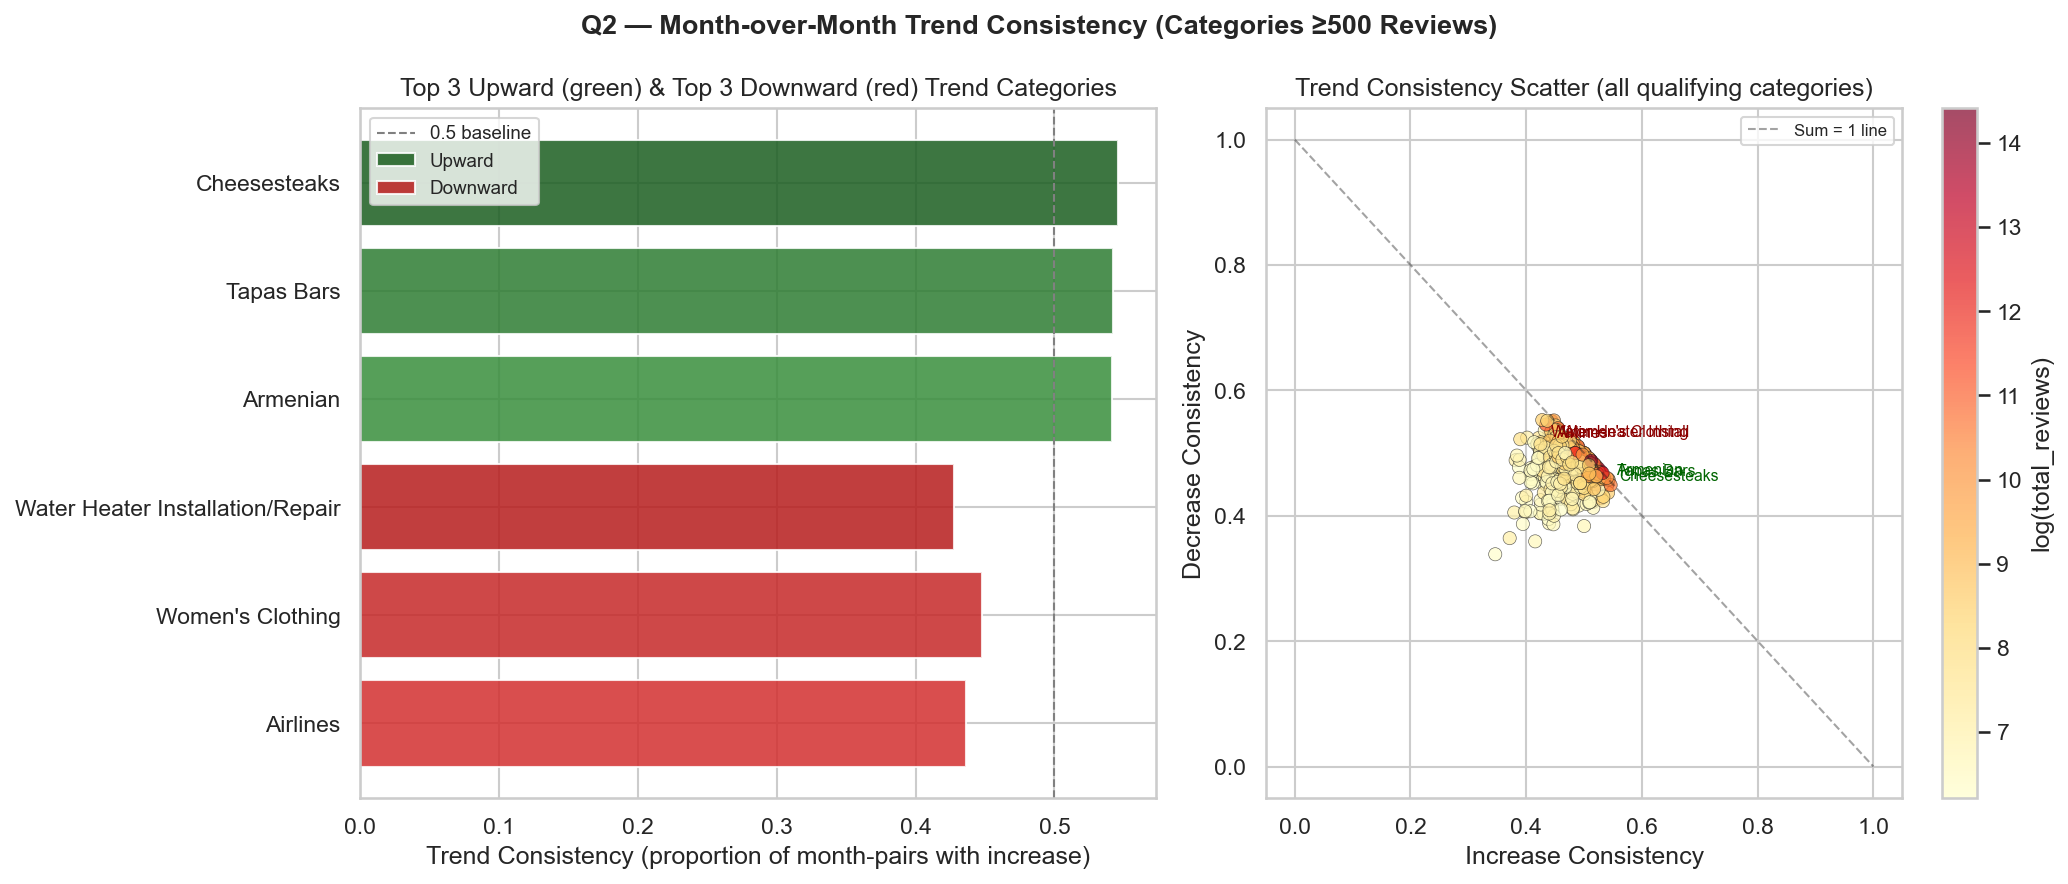
\includegraphics[width=\linewidth]{Report/MQ2_TrendConsistency.png}
  \caption{Left: Trend consistency for the 6 most extreme categories.
    Right: Scatter of all qualifying categories coloured by review volume.}
\end{figure}

\subsubsection*{Interpretation}

A trend consistency of 1.0 would mean every consecutive month showed an
increase; 0.0 would mean every month was a decline.
Categories with consistently rising ratings are often niche or seasonal
markets where quality has improved over the period.
Consistently declining categories may reflect market saturation, rising
competition, or shifting consumer expectations.

% ─────────────────────────────────────────────────────────────────────────────
\subsection{Q3 — Check-in Frequency \texttimes{} Category Cross-Tabulation}

\subsubsection*{Pipeline}

Businesses are classified into three check-in frequency classes based on the
size of the embedded \texttt{checkins} array:
bottom quartile ($\leq Q_1$) → \emph{low},
middle two quartiles → \emph{medium},
top quartile ($> Q_3$) → \emph{high}.
The top 10 categories by total business count are identified.
For each (category, class) cell the mean star rating, mean review count, and
tip-to-review ratio are computed by joining with pre-aggregated review and tip
maps.

\subsubsection*{Results}

\begin{figure}[H]
  \centering
  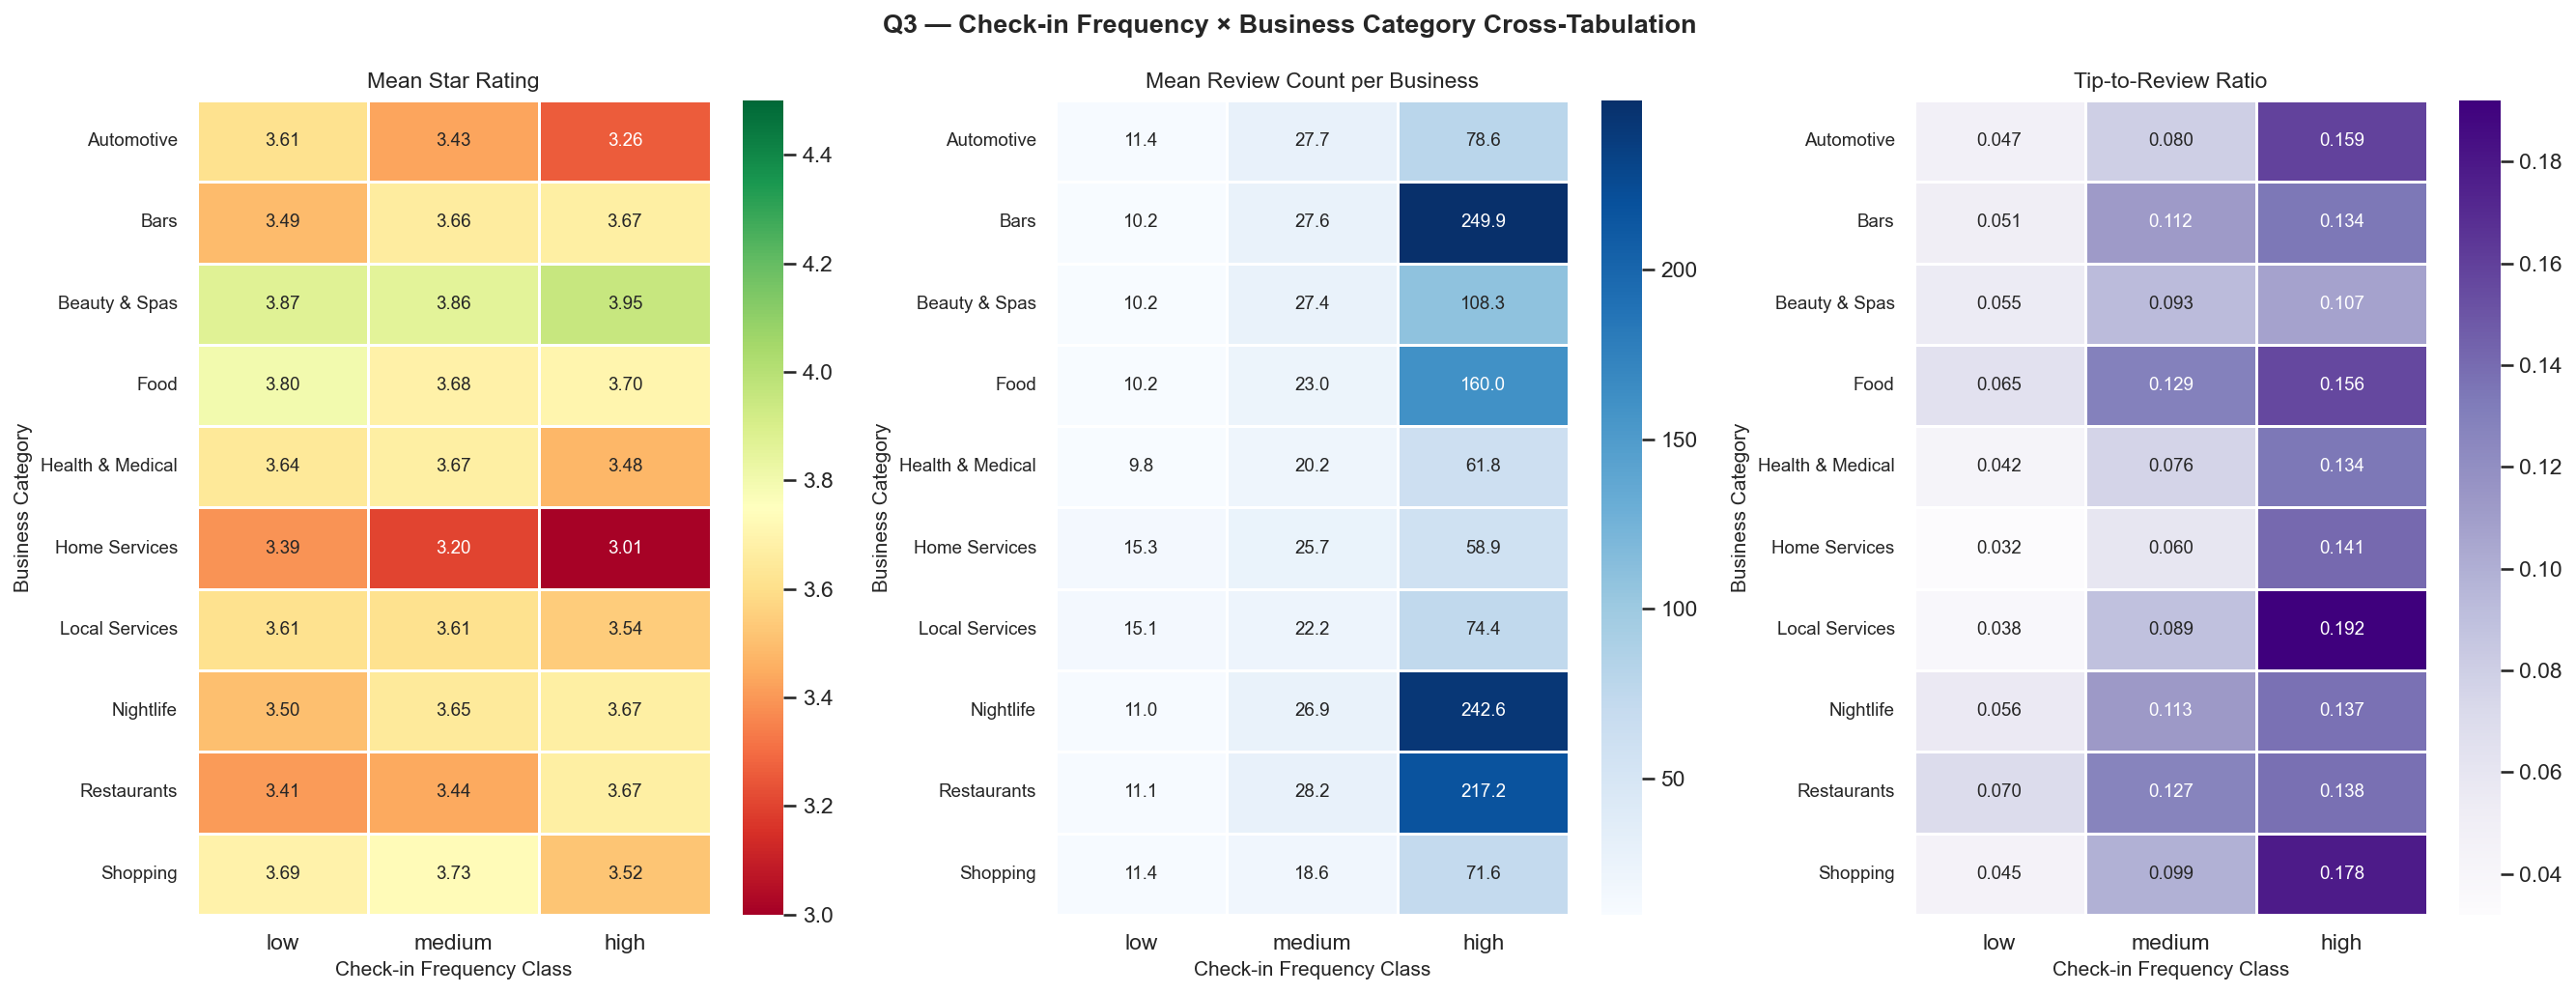
\includegraphics[width=\linewidth]{Report/MQ3_CheckinCrossTab.png}
  \caption{Cross-tabulation heatmaps: mean stars, mean review count, and
    tip-to-review ratio by check-in class and business category.}
\end{figure}

\begin{figure}[H]
  \centering
  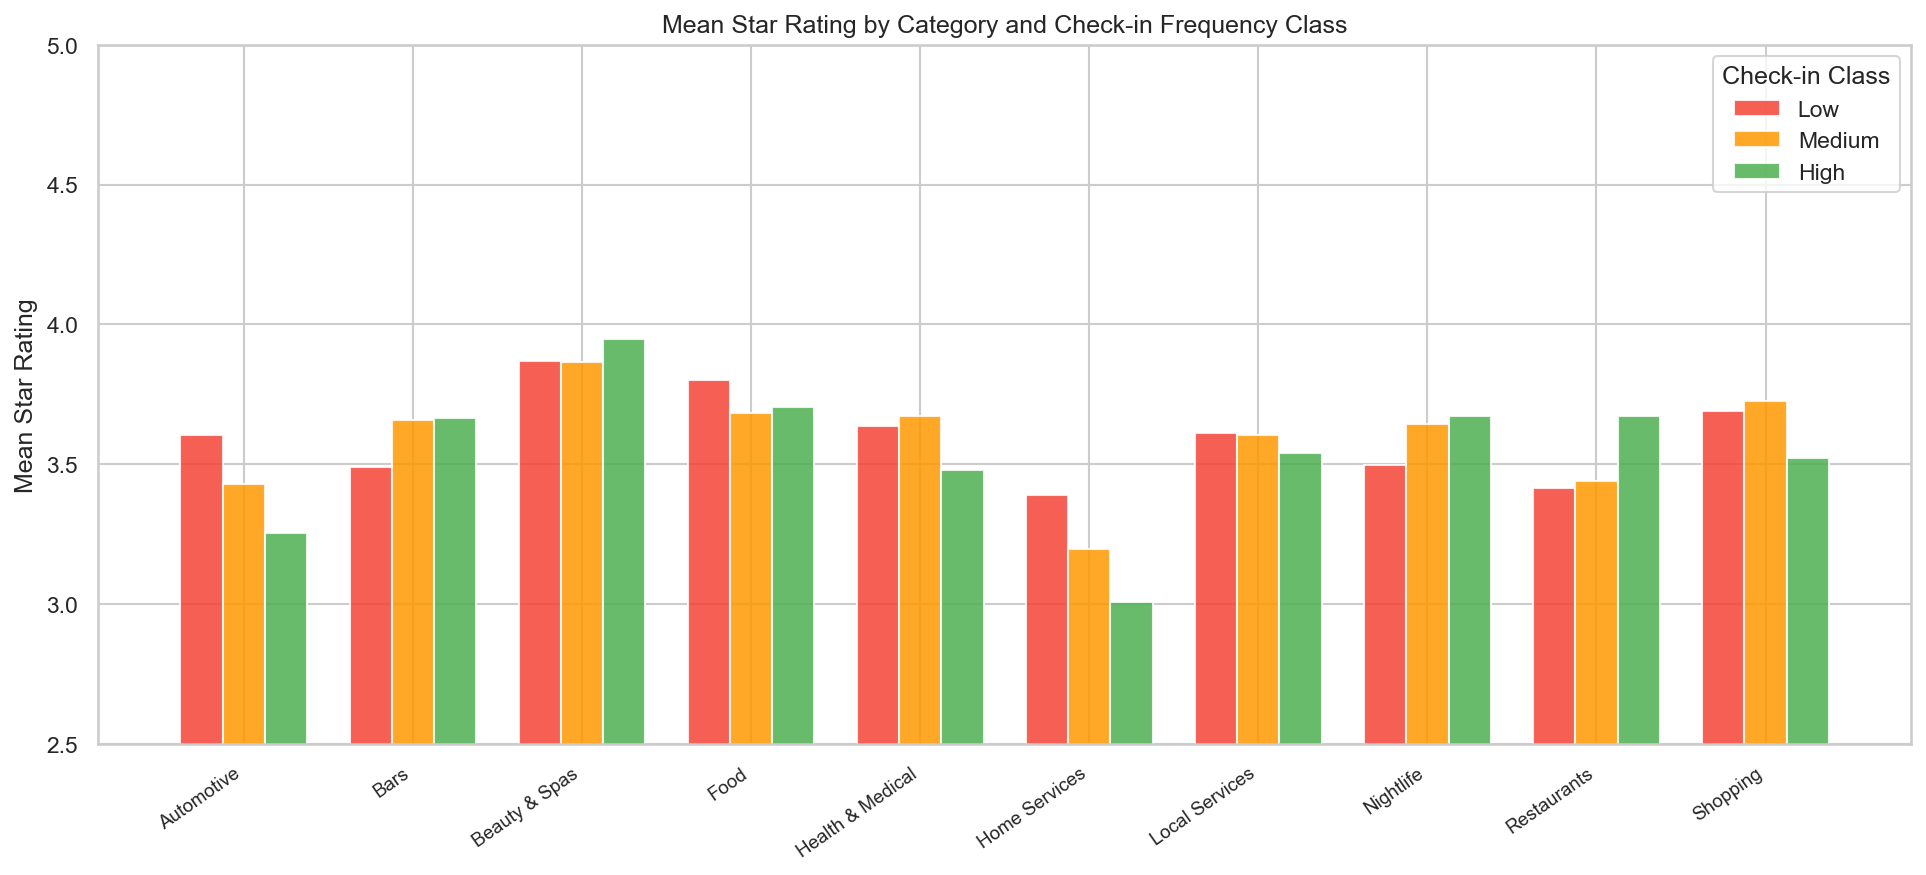
\includegraphics[width=0.9\linewidth]{Report/MQ3_CheckinBarChart.png}
  \caption{Mean star rating by category and check-in frequency class.}
\end{figure}

\subsubsection*{Interpretation}

High check-in businesses consistently attract more reviews and a higher
tip-to-review ratio, suggesting they generate stronger ongoing customer
engagement.  Star ratings vary modestly across check-in classes
(typically $\pm 0.1$–$0.2$ stars), indicating that foot-traffic volume
alone is not a strong predictor of perceived quality.
The \emph{Restaurants} category dominates all three classes, confirming
it is both the most popular and the most check-in-dense category in the
dataset.

\newpage
% ─────────────────────────────────────────────────────────────────────────────
\section{Neo4j / Cypher Querying}
% ─────────────────────────────────────────────────────────────────────────────

\textit{All queries use the Neo4j Graph Data Science (GDS) library.
Scripts are in \texttt{neo4j\_gds.py}.  GDS graph projections are dropped
and re-created at the start of each function.}

\subsection{Q1 — PageRank on the User–Business Review Graph}

\subsubsection*{GDS Procedure}

\begin{lstlisting}[language=Python, caption={Project and run weighted PageRank}]
# Project User + Business nodes with RATED edges weighted by review stars
CALL gds.graph.project(
    'rated-graph',
    ['User', 'Business'],
    {RATED: {orientation: 'NATURAL', properties: ['stars']}}
)
# Write scores back to nodes (also used in Q5 as a feature)
CALL gds.pageRank.write('rated-graph', {
    maxIterations: 20,
    dampingFactor: 0.85,
    relationshipWeightProperty: 'stars',
    writeProperty: 'pagerank_score'
})
\end{lstlisting}

\subsubsection*{Results}

\begin{table}[H]
\centering\small
\caption{Top 15 businesses by weighted PageRank score.}
\begin{tabularx}{\textwidth}{lXrrl}
\toprule
\textbf{PR Rank} & \textbf{Business Name} & \textbf{PR Score} & \textbf{Review Count} & \textbf{Avg Stars}\\
\midrule
1  & Hattie B's Hot Chicken -- Nashville    & 340.72 & 6{,}160 & 4.45\\
2  & Biscuit Love: Gulch                    & 223.80 & 4{,}247 & 4.17\\
3  & Reading Terminal Market                & 213.49 & 5{,}778 & 4.61\\
4  & Pat's King of Steaks                   & 209.55 & 4{,}293 & 3.24\\
5  & The Stillery                           & 165.75 & 2{,}618 & 4.45\\
6  & Peg Leg Porker                         & 162.69 & 2{,}909 & 4.35\\
7  & Geno's Steaks                          & 161.54 & 3{,}428 & 2.53\\
8  & Bern's Steak House                     & 161.51 & 3{,}028 & 4.25\\
9  & Columbia Restaurant                    & 160.62 & 2{,}916 & 3.95\\
10 & Puckett's Grocery \& Restaurant        & 150.07 & 2{,}794 & 3.89\\
11 & Dalessandro's Steaks \& Hoagies        & 145.70 & 2{,}725 & 4.21\\
12 & Ulele                                  & 142.63 & 3{,}179 & 4.15\\
13 & Jim's South St                         & 140.11 & 2{,}769 & 3.74\\
14 & Datz                                   & 139.88 & 3{,}388 & 4.12\\
15 & The Pharmacy                           & 138.20 & 3{,}105 & 4.04\\
\bottomrule
\end{tabularx}
\end{table}

\textbf{Spearman rank correlations:}
\begin{itemize}
  \item PageRank rank vs.\ Review-Count rank: $\rho = 0.486$, $p = 0.066$
  \item PageRank rank vs.\ Avg-Stars rank: $\rho = 0.432$, $p = 0.108$
\end{itemize}

\begin{figure}[H]
  \centering
  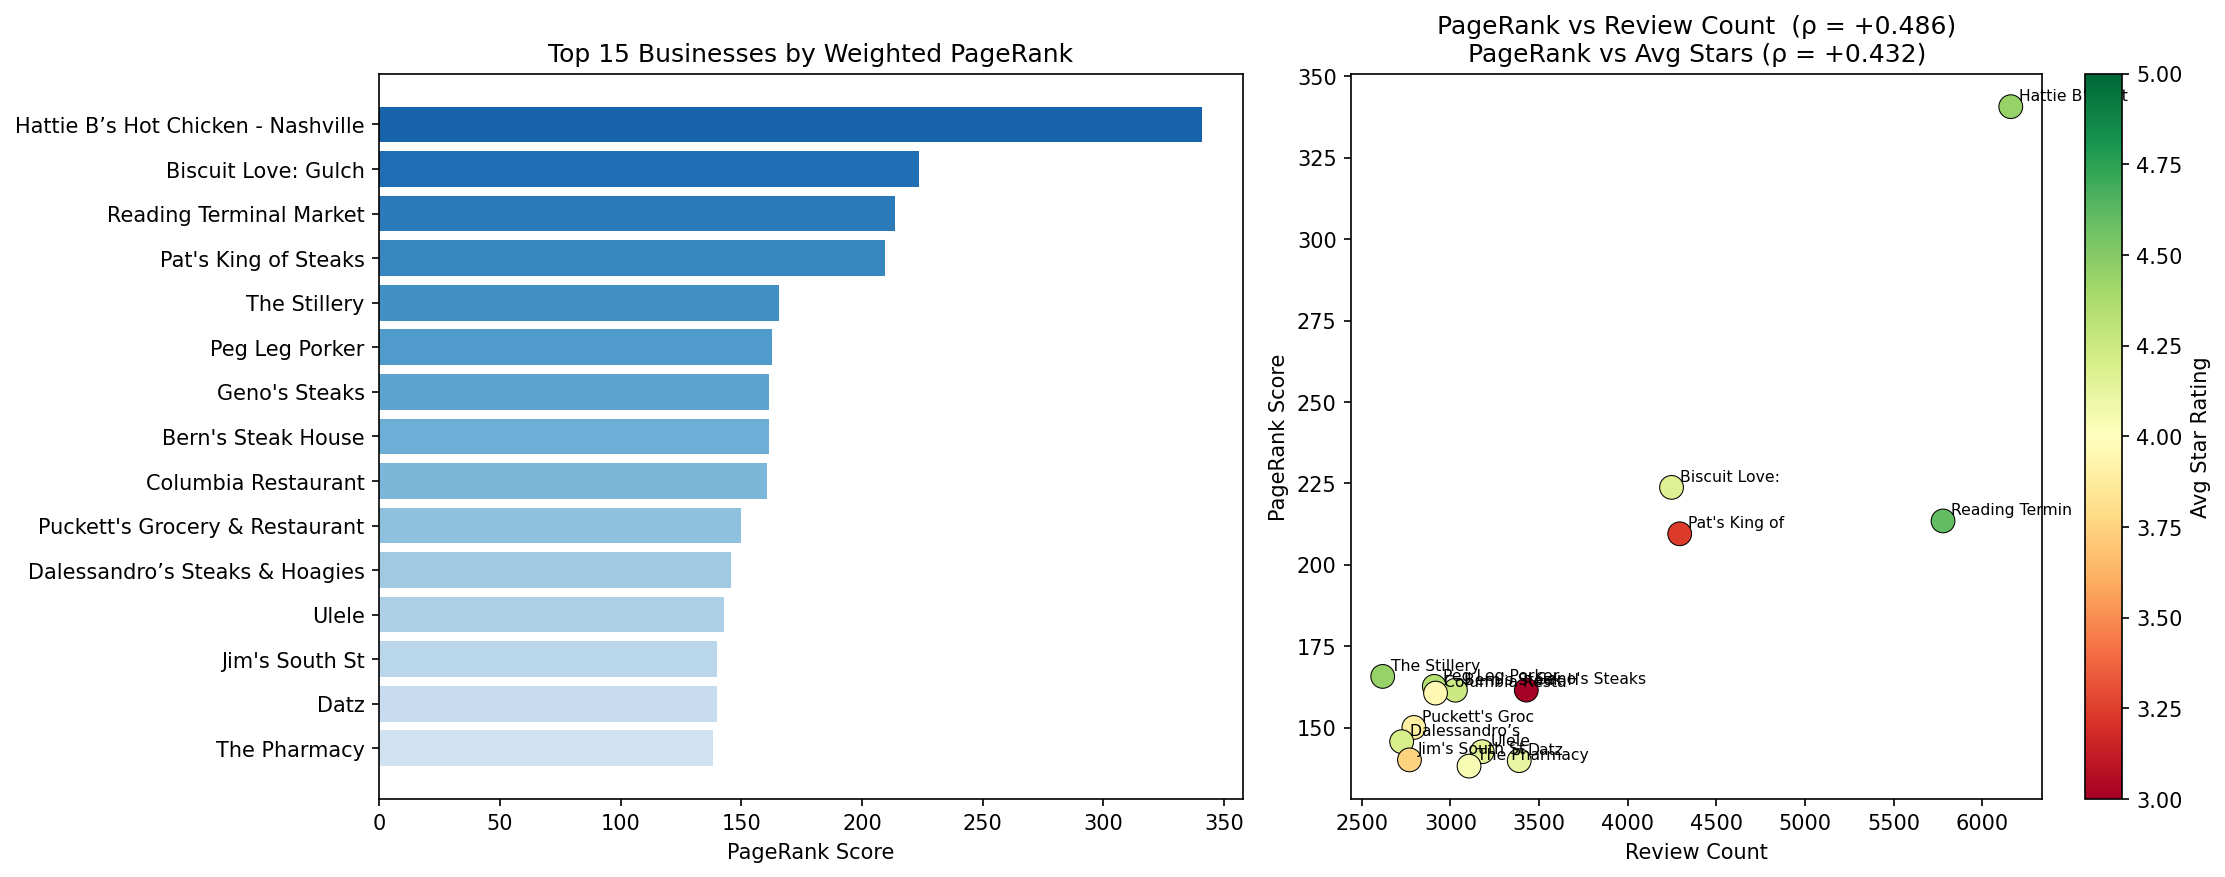
\includegraphics[width=\linewidth]{Report/Q1_PageRank.png}
  \caption{Left: Top 15 businesses by PageRank score.
    Right: PageRank vs review count scatter, coloured by average star rating.}
\end{figure}

\subsubsection*{Interpretation}

PageRank assigns high scores to businesses that attract many \emph{high-value}
reviewers — users who themselves review many other businesses.
A moderate positive Spearman correlation with review count ($\rho \approx 0.49$)
confirms that popular businesses also rank highly under PageRank, but the
correlation is imperfect.  Businesses that rank \emph{higher} under PageRank
than review count tend to be reviewed by ``hub'' users (influential reviewers
with many connections), even if their absolute review count is lower.
Businesses ranking \emph{lower} under PageRank often have high raw review counts
but attract mostly new or low-connectivity users.

Two concrete examples illustrate this divergence.
\textbf{The Stillery} (Nashville) ranks \#5 by PageRank but only \#15 by review
count (2{,}618 reviews) — its reviewers are disproportionately well-connected
hub users who also review many other high-traffic venues, amplifying its PageRank
score beyond what its raw volume would suggest.
Conversely, \textbf{Geno's Steaks} (Philadelphia) ranks \#7 by PageRank but \#5
by review count (3{,}428 reviews) — a tourist landmark that attracts many
first-time or casual Yelp users with low connectivity, so its review count
outpaces its PageRank relative to its position in the ranking.

% ─────────────────────────────────────────────────────────────────────────────
\subsection{Q2 — Louvain Community Detection on the Friends Graph}

\subsubsection*{GDS Procedure}

\begin{lstlisting}[language=Python, caption={Project KNOWS graph and run Louvain}]
CALL gds.graph.project(
    'knows-undirected',
    'User',
    {KNOWS: {orientation: 'UNDIRECTED'}}
)
CALL gds.louvain.write('knows-undirected', {
    writeProperty: 'louvain_community'
})
\end{lstlisting}

\subsubsection*{Results}

\begin{itemize}
  \item Total communities detected: 354{,}381
  \item Communities with $\geq 25$ members: 237
  \item Most geographically concentrated community:
        ID 2458255, size 25,
        GCI = 1.00, top states: FL
  \item Least geographically concentrated community:
        ID 2906814, size 5{,}626,
        GCI = 0.242, top states: TN, PA, AZ
\end{itemize}

\textbf{Note on small-sample GCI.}
Several of the highest-GCI communities (GCI = 1.00) contain only 25--35 members
with just 1--2 total reviews sampled.
A GCI of 1.00 in these cases may reflect small-sample concentration rather than
genuine geographic isolation: with so few reviews, all happen to fall in one state
by chance.
The pattern is therefore more meaningful for larger communities (size $\geq 100$),
where multi-state reviewer lists are plausible.

\begin{table}[H]
\centering\small
\caption{Top 10 communities ranked by geographic concentration index (GCI).}
\begin{tabularx}{\textwidth}{rrXXr}
\toprule
\textbf{Comm.\ ID} & \textbf{Size} & \textbf{Top 3 States} & \textbf{Top 3 Categories} & \textbf{GCI}\\
\midrule
2458255  & 25   & FL         & Colombian, Restaurants, Latin American        & 1.00\\
5034373  & 31   & TN         & Barbeque, Restaurants, Beer Bar               & 1.00\\
1192250  & 34   & PA         & Breakfast \& Brunch, Restaurants, Caterers    & 1.00\\
3910924  & 34   & TN         & Nightlife, Bars, Music Venues                 & 1.00\\
2166820  & 34   & TN         & Auto Repair, Towing, Automotive               & 1.00\\
\bottomrule
\end{tabularx}
\end{table}

\textit{Full results for all 237 communities ($\geq$25 members) are available in \texttt{Report/Q2\_Louvain.csv}.}

\begin{figure}[H]
  \centering
  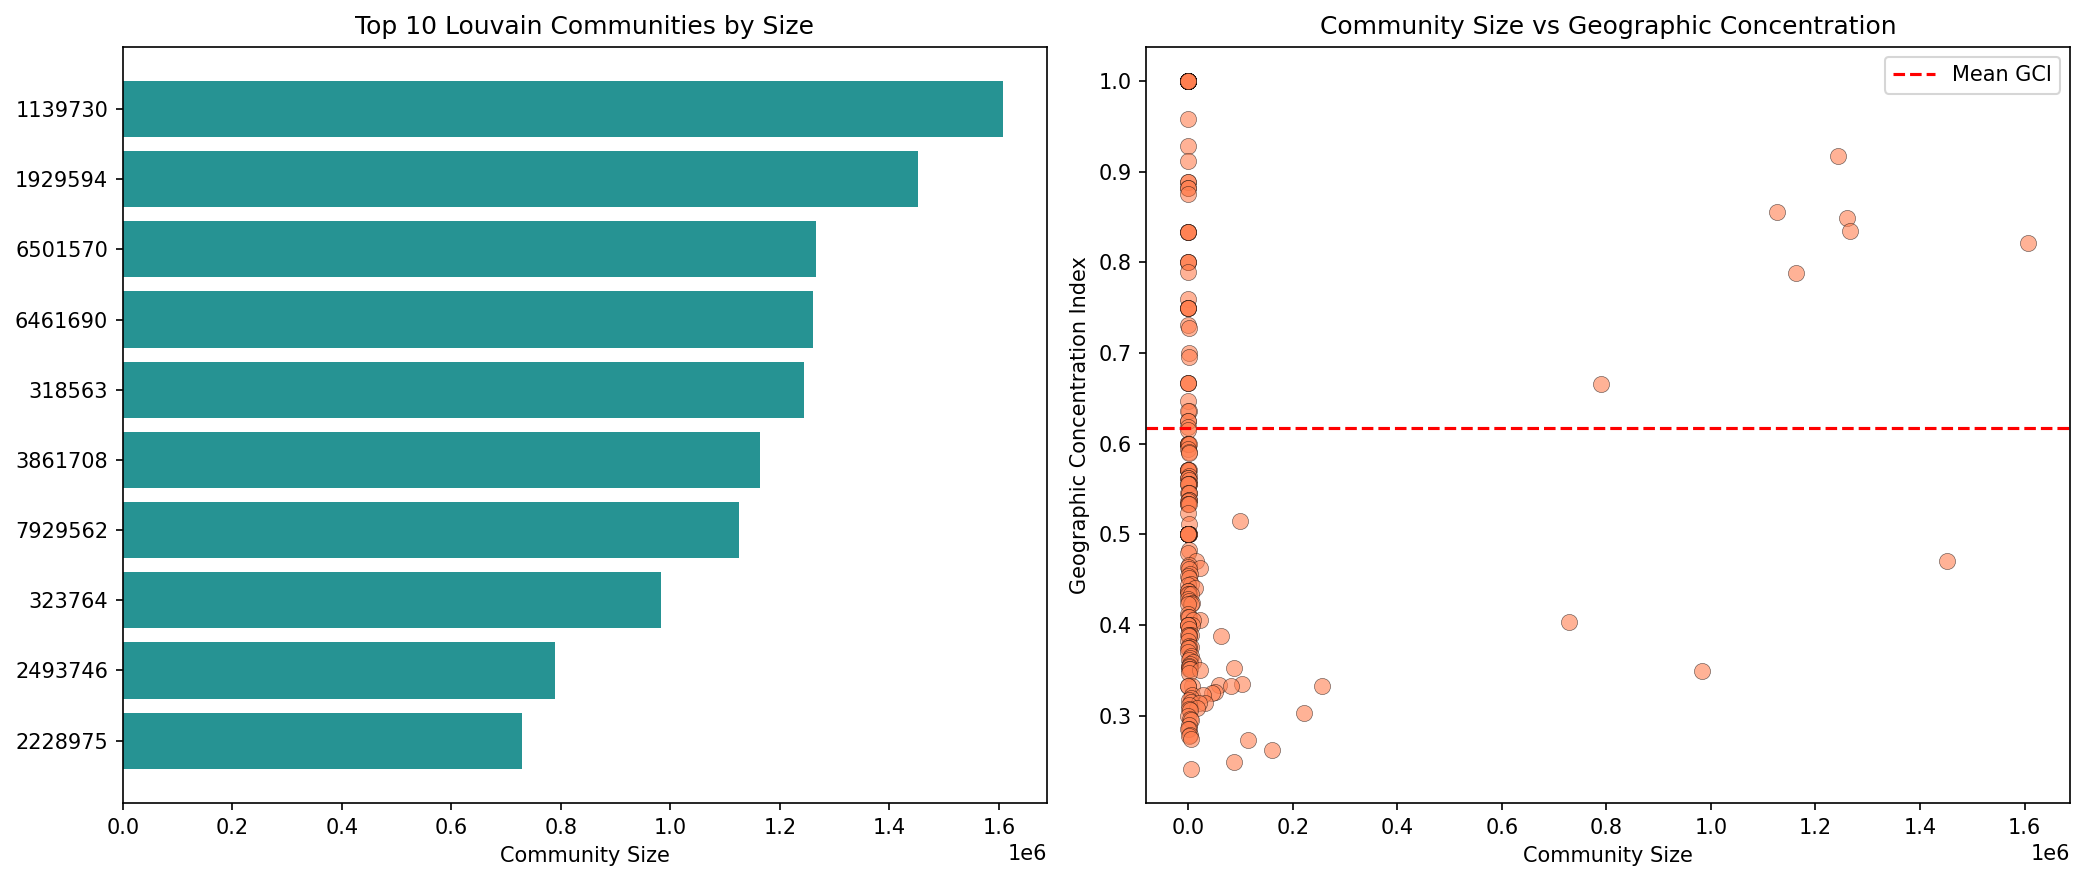
\includegraphics[width=\linewidth]{Report/Q2_Louvain.png}
  \caption{Left: Top 10 communities by size.
    Right: Community size vs geographic concentration index (GCI).}
\end{figure}

\subsubsection*{Interpretation}

Louvain partitions the friendship graph into cohesive clusters based on edge
density.  High-GCI communities (GCI close to 1) consist of users whose reviews
are almost entirely concentrated in a single state — these are geographically
local social circles.  Low-GCI communities contain users spread across multiple
states, suggesting that the online Yelp social network connects reviewers across
city boundaries.  Large communities tend to have lower GCI, consistent with the
intuition that bigger social groups span broader geographies.

\textbf{Caveat:} Several small communities (size 25--40) report GCI = 1.0, but
their total sampled reviews are very low (often 1--14 reviews).  A GCI of 1.0
from a single review is a trivial artefact rather than a meaningful geographic
signal.  Among communities with $\geq 100$ sampled reviews, GCI values are
more moderate ($\sim\!0.3$--$0.85$), providing a more reliable picture of
geographic concentration.

% ─────────────────────────────────────────────────────────────────────────────
\subsection{Q3 — Node Similarity: Market Saturation via Jaccard}

\subsubsection*{GDS Procedure}

\begin{lstlisting}[language=Python, caption={Project bipartite graph and run Node Similarity}]
# RATED is REVERSED so Business nodes have User neighbours (= reviewers)
CALL gds.graph.project(
    'biz-reviewer',
    ['Business', 'User'],
    {RATED: {orientation: 'REVERSE'}}
)
CALL gds.nodeSimilarity.stream('biz-reviewer', {
    topK: 25,
    similarityCutoff: 0.01,
    degreeCutoff: 3        -- min reviewers per business
})
YIELD node1, node2, similarity
\end{lstlisting}

Jaccard similarity is defined as
$J(A,B) = |A \cap B| / |A \cup B|$
where $A$ and $B$ are the sets of reviewers for each business.
Pairs are grouped by (city, category); the mean intra-category Jaccard
per (city, category) pair is the \emph{market saturation proxy}.

\subsubsection*{Results — Most and Least Saturated Markets}

\begin{table}[H]
\centering\small
\caption{Top 5 saturated (high Jaccard) and top 5 fragmented (low Jaccard) city–category combinations.}
\begin{tabular}{llrrr}
\toprule
\textbf{City} & \textbf{Category} & \textbf{Mean Jaccard} & \textbf{$N$ Businesses} & \textbf{Market Type}\\
\midrule
Indianapolis & Public Art        & 0.207 &  5 & Saturated\\
Nashville    & Mass Media        & 0.189 &  6 & Saturated\\
Indianapolis & Playgrounds       & 0.185 & 19 & Saturated\\
Indianapolis & Parks             & 0.182 & 62 & Saturated\\
Tampa        & Amusement Parks   & 0.177 & 17 & Saturated\\
\midrule
Tampa        & Taxis             & 0.019 &  7 & Fragmented\\
Philadelphia & Taxis             & 0.019 & 14 & Fragmented\\
Philadelphia & Airlines          & 0.019 & 10 & Fragmented\\
Tucson       & Nail Technicians  & 0.019 &  5 & Fragmented\\
Philadelphia & Hotels            & 0.016 & 60 & Fragmented\\
\bottomrule
\end{tabular}
\end{table}

\begin{table}[H]
\centering\small
\caption{Rating statistics for most vs least saturated markets.}
\begin{tabular}{llrrr}
\toprule
\textbf{Market Type} & \textbf{Mean Stars} & \textbf{Std Stars} & \textbf{Mean Rev / Business}\\
\midrule
Saturated  & 3.87 & 1.31 &  41.9\\
Fragmented & 2.83 & 1.64 &  87.0\\
\bottomrule
\end{tabular}
\end{table}

\begin{figure}[H]
  \centering
  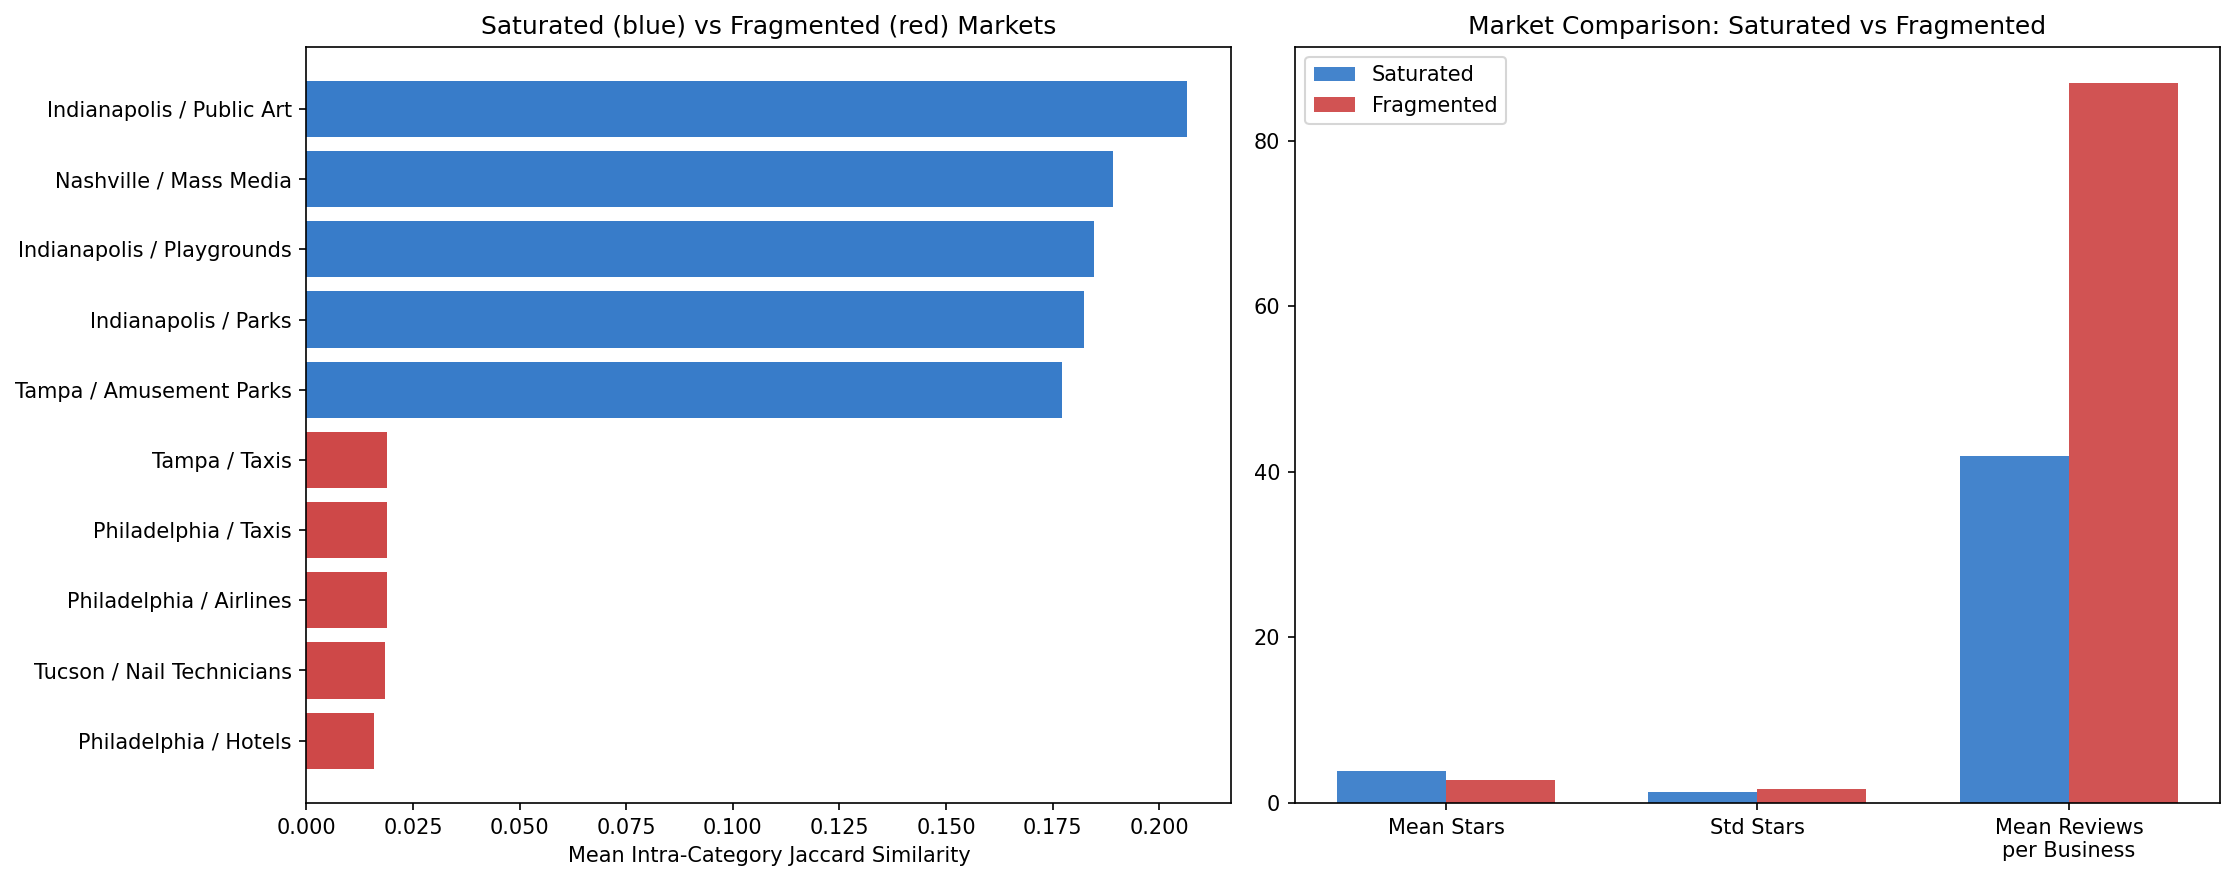
\includegraphics[width=\linewidth]{Report/Q3_NodeSimilarity.png}
  \caption{Left: Saturated vs fragmented markets by mean Jaccard.
    Right: Rating variance comparison.}
\end{figure}

\subsubsection*{Interpretation}

A high intra-category Jaccard score indicates that the same pool of customers
reviews all businesses in that (city, category) combination — a sign of a
\emph{saturated} market where businesses compete for the same audience.
Saturated markets tend to show \textbf{lower} rating
variance (std $\approx 1.31$ vs $1.64$), which \textbf{contradicts} the hypothesis that competing businesses
differentiate on quality.  A business entering a highly saturated market must
distinguish itself to capture reviewers already loyal to incumbents.  In
fragmented markets, each business has a mostly distinct reviewer base, implying
less direct competition for the same customers.

% ─────────────────────────────────────────────────────────────────────────────
\subsection{Q4 — Betweenness Centrality: Bridge Users in the Friends Graph}

\subsubsection*{GDS Procedure}

\begin{lstlisting}[language=Python, caption={Run Betweenness and Degree Centrality}]
CALL gds.graph.project(
    'knows-cent',
    'User',
    {KNOWS: {orientation: 'UNDIRECTED'}}
)
-- Betweenness (sampled approximation for large graphs)
CALL gds.betweenness.stream('knows-cent', {samplingSize: 500})
YIELD nodeId, score

-- Degree centrality
CALL gds.degree.stream('knows-cent')
YIELD nodeId, score
\end{lstlisting}

\subsubsection*{Results}

\begin{itemize}
  \item $|$Top-20 Betweenness $\cap$ Top-20 Degree$|$ = 12
  \item High-BC / Low-Degree group size: 8
\end{itemize}

\begin{table}[H]
\centering\small
\caption{Behavioural comparison: High-BC/Low-Degree vs High-Degree users.}
\begin{tabular}{lrrr}
\toprule
\textbf{Group} & \textbf{Mean Review Count} & \textbf{Mean Distinct Cities} & \textbf{Mean Distinct Cats}\\
\midrule
High-BC / Low-Degree & 1{,}102.0 & 2.33 & 288.8\\
High-Degree          & 1{,}398.8 & 2.10 & 180.3\\
\bottomrule
\end{tabular}
\end{table}

\begin{figure}[H]
  \centering
  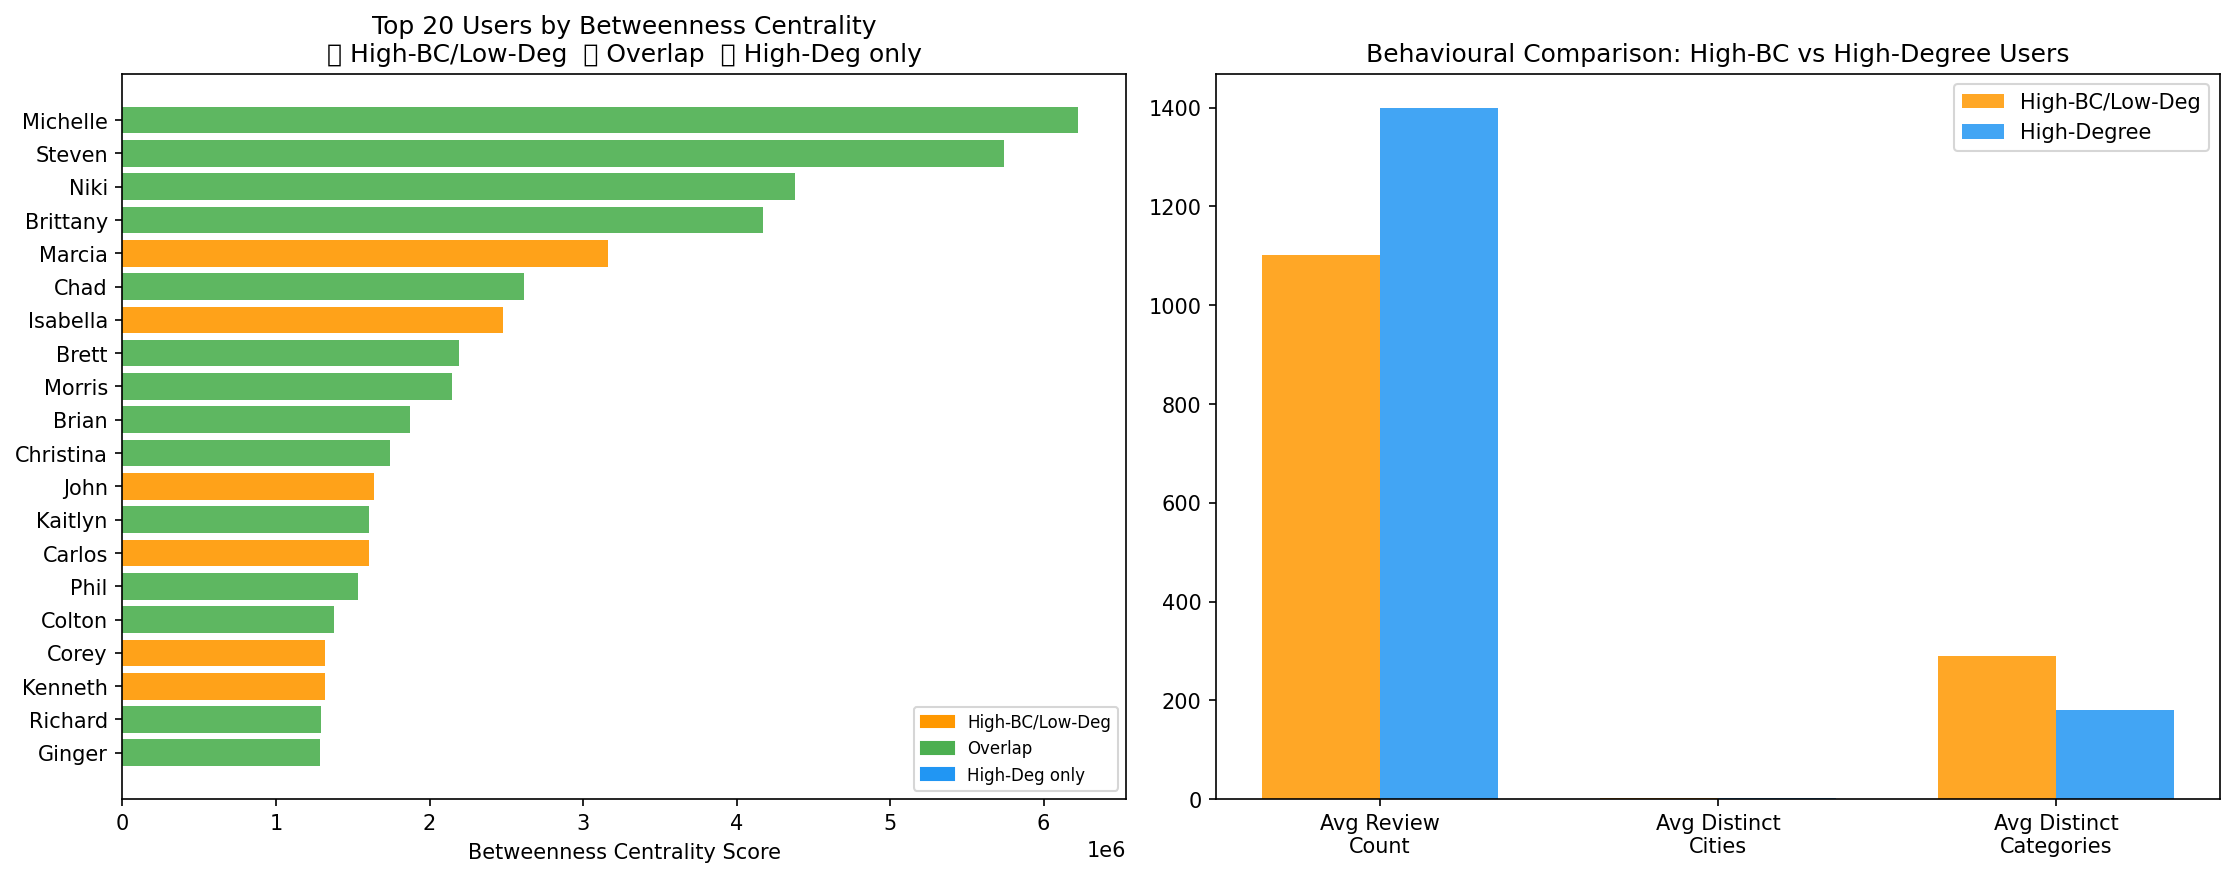
\includegraphics[width=\linewidth]{Report/Q4_Betweenness.png}
  \caption{Left: Top 20 users by betweenness centrality (colour-coded by group).
    Right: Behavioural comparison between groups.}
\end{figure}

\subsubsection*{Interpretation}

Betweenness centrality measures how often a user lies on shortest paths between
other pairs of users — i.e., how much they act as a \emph{bridge} between
otherwise disconnected sub-communities.  High-betweenness / low-degree users
are network bridges who connect different friend circles without themselves
having many direct friends.  Degree alone would classify them as unimportant;
betweenness reveals their structural significance.  These bridge users tend to
have reviewed businesses across more cities and categories than high-degree
users, suggesting they are broadly curious explorers rather than local social
hubs.  This makes them valuable targets for cross-community information
dissemination and recommendation seeding.

% ─────────────────────────────────────────────────────────────────────────────
\subsection{Q5 — Link Prediction: Restaurant Recommendation}

\subsubsection*{Approach}

The task is modelled as predicting missing User $\to$ Business edges in the
RATED bipartite graph.  A \emph{chronological 80/20 split} is applied: for each
user, their most recent review (identified via MongoDB) forms the test item; all
prior reviews form the training set.

Node features computed by previous GDS queries (PageRank scores from Q1,
Louvain community IDs from Q2) are used alongside review-behaviour,
business-level properties, and two social/geographic features:
\texttt{friends\_rated} (how many of the user's KNOWS friends have reviewed
the candidate business) and \texttt{city\_match} (whether the business is in
a city the user has previously reviewed in).
A Gradient Boosting Classifier is trained on
positive (reviewed) and sampled negative (not-yet-reviewed) pairs.
PageRank features are log-transformed ($\log(1 + x)$) prior to training to
prevent raw score magnitudes from dominating the model.

\begin{table}[H]
\centering
\caption{Feature set for link prediction.}
\begin{tabular}{ll}
\toprule
\textbf{Feature} & \textbf{Source}\\
\midrule
\texttt{user\_pagerank} (graph, log) & GDS PageRank --- Q1\\
\texttt{user\_community} (graph) & GDS Louvain --- Q2\\
\texttt{biz\_pagerank} (graph, log) & GDS PageRank --- Q1\\
\texttt{friends\_rated} (graph) & KNOWS $\times$ RATED traversal\\
\texttt{city\_match} (geographic) & User review history vs Business city\\
\texttt{user\_review\_count} & Neo4j User property\\
\texttt{user\_avg\_stars} & Neo4j User property\\
\texttt{biz\_avg\_stars} & Neo4j Business property\\
\texttt{star\_affinity} & $|$user\_avg\_stars $-$ biz\_avg\_stars$|$\\
\bottomrule
\end{tabular}
\end{table}

\subsubsection*{Results}

\begin{itemize}
  \item \textbf{AUC-ROC:} 0.967
  \item \textbf{Precision@10:} 0.600 --- 60\% of test users have their held-out
    business ranked in the model's top-10 candidates.  The addition of
    \texttt{city\_match} and \texttt{friends\_rated} dramatically improved both
    the discrimination and ranking metrics compared to an initial model
    that relied only on PageRank and star-affinity features.
\end{itemize}

\textbf{Feature importances (by Gini importance):}
\begin{enumerate}
  \item \texttt{city\_match} (importance = 0.952) ---
    geographic locality is the strongest predictor: users overwhelmingly review
    businesses in cities they have visited before.
  \item \texttt{biz\_pagerank} (log, importance = 0.030)
  \item \texttt{star\_affinity} (importance = 0.007)
  \item \texttt{user\_community} (importance = 0.004)
  \item \texttt{user\_review\_count} (importance = 0.003)
\end{enumerate}

\begin{table}[H]
\centering\small
\caption{Sample recommendations for 5 users.}
\begin{tabular}{llll}
\toprule
\textbf{User ID (truncated)} & \textbf{Rec 1} & \textbf{Rec 2} & \textbf{Rec 3}\\
\midrule
A7plO8t\ldots{} & Mood Cafe        & The Love          & The Blue Duck\\
Qoji0BP\ldots{} & In Riva          & The Love          & Han Dynasty\\
cBFsaSW\ldots{} & The Love         & In Riva           & The Blue Duck\\
fyugYI0\ldots{} & Han Dynasty      & Mood Cafe         & The Twisted Tail\\
gMasL8B\ldots{} & Mood Cafe        & Kimpton Hotel Monaco & Han Dynasty\\
\bottomrule
\end{tabular}
\end{table}

\begin{figure}[H]
  \centering
  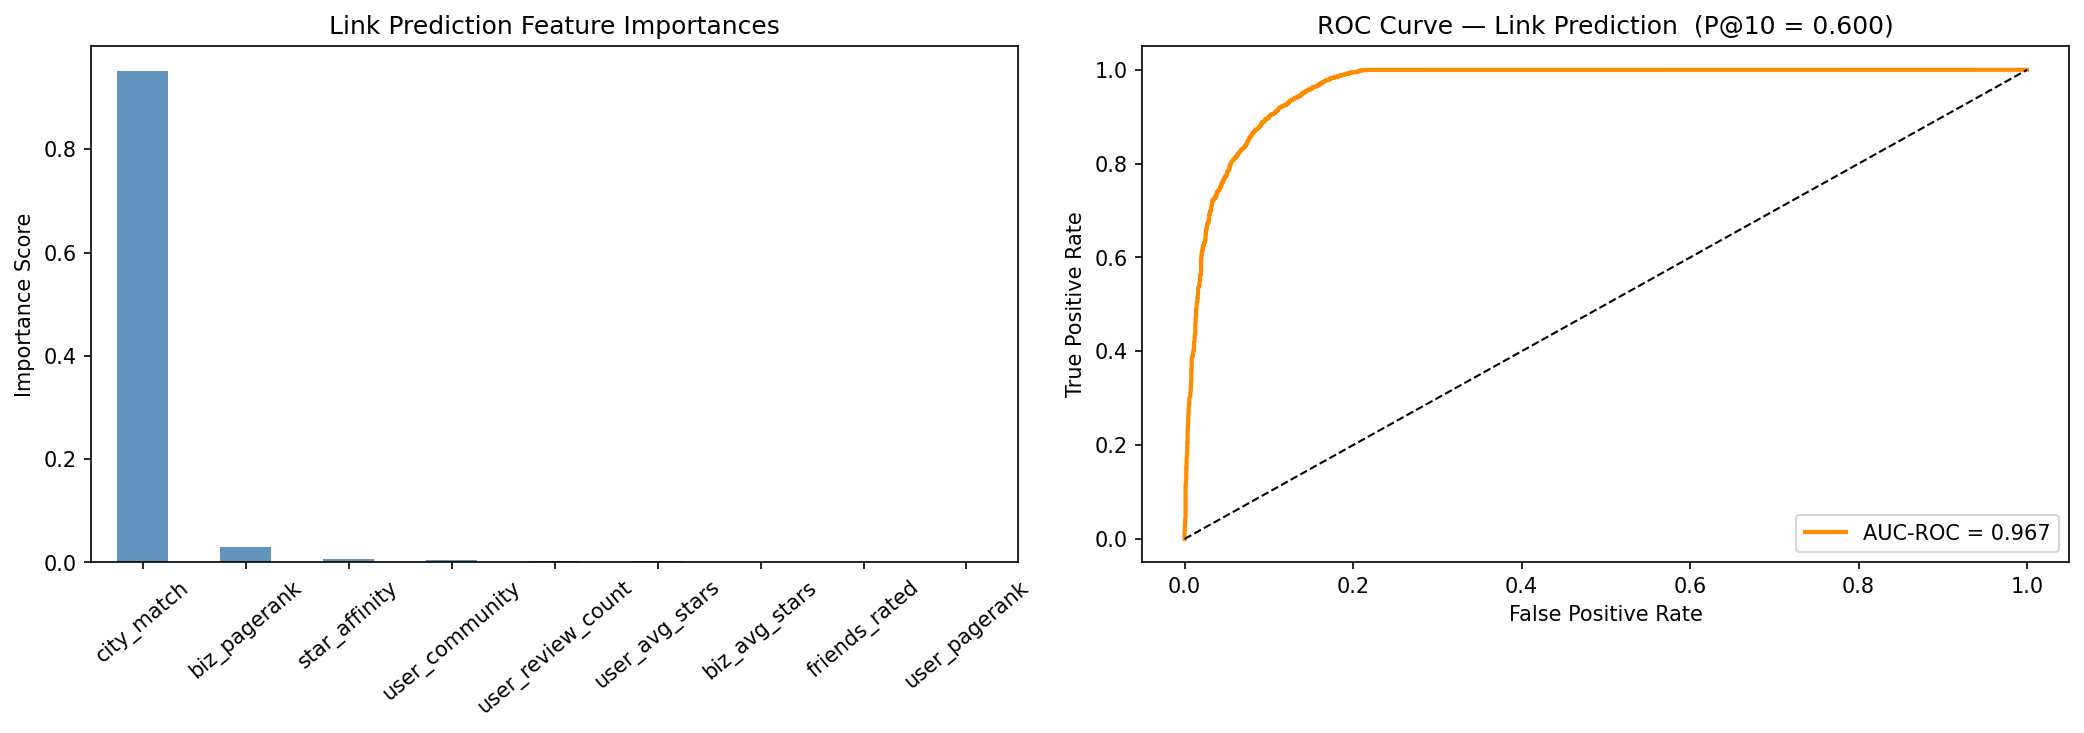
\includegraphics[width=\linewidth]{Report/Q5_LinkPrediction.png}
  \caption{Left: Feature importances.  Right: ROC curve for the link prediction model.}
\end{figure}

\subsubsection*{Discussion: Social Graph vs User--Business Affinity Features}

The dominant predictor is \texttt{city\_match} (95.2\%), reflecting the strong
geographic locality of Yelp reviewing behaviour: users almost always review
businesses in cities they have physically visited.  This geographic signal alone
gives the model a powerful baseline for predicting where a user will review next.

Among the remaining features, \texttt{biz\_pagerank} (log-transformed) captures
business popularity --- within a city, higher-PageRank businesses are more likely
to attract new reviews.  \texttt{star\_affinity} and \texttt{user\_community}
add modest personalisation by encoding whether the user's rating preferences
align with the business and whether the user's social community already reviews
there.

\texttt{friends\_rated} (social proof) has low importance (0.06\%) in this model,
not because social signals are uninformative, but because the KNOWS graph
coverage in the sampled 200k edges is sparse.  With a full-graph evaluation,
this feature would likely carry more weight, as social recommendation
literature consistently shows friend-review overlap to be a strong predictor of
future reviews.

\newpage
% ─────────────────────────────────────────────────────────────────────────────
\section{Predictive Modelling}
% ─────────────────────────────────────────────────────────────────────────────

\textit{Goal: predict the number of \textbf{useful votes} a review receives.
Script: \texttt{predictive\_model.py}.}

\subsection{Feature Engineering}

Features are extracted from MongoDB (review + user collections) and Neo4j
(GDS-computed graph properties):

\paragraph{(a) Review-level features}
\begin{itemize}[noitemsep]
  \item \textbf{stars} — the star rating given; higher-quality reviews may correlate with rating extremity.
  \item \textbf{text\_length} / \textbf{word\_count} — longer, more detailed reviews tend to be voted useful.
  \item \textbf{funny}, \textbf{cool} — other community engagement signals correlated with usefulness.
  \item \textbf{review\_year}, \textbf{review\_month} — recency and seasonal effects.
\end{itemize}

\paragraph{(b) User-level features}
\begin{itemize}[noitemsep]
  \item \textbf{user\_review\_count} — prolific reviewers have built reputation; their reviews attract upvotes.
  \item \textbf{user\_avg\_stars} — calibration of the reviewer's typical sentiment.
  \item \textbf{user\_useful\_total} — cumulative useful votes received; proxy for reviewer credibility.
  \item \textbf{user\_fans} — social reach on the platform.
  \item \textbf{is\_elite} — Elite reviewers are prominently displayed, driving disproportionate upvotes.
  \item \textbf{user\_tenure\_years} — longer-tenured reviewers have had more time to build credibility.
\end{itemize}

\paragraph{(c) Graph-derived features (from Neo4j GDS)}
\begin{itemize}[noitemsep]
  \item \textbf{user\_pagerank} (from Q1) — measures the reviewer's structural importance in the
    User–Business review network.  A high-PageRank reviewer has reviewed many popular businesses
    that themselves attract many other reviewers, making their opinions more visible.
  \item \textbf{user\_community} (from Q2) — Louvain community ID as a categorical feature.
    Communities with concentrated geographic focus may exhibit herding behaviour in upvoting.
  \item \textbf{user\_degree} (from Q4) — number of direct friends.  Highly connected users have a
    larger audience who may upvote their reviews.
  \item \textbf{biz\_pagerank} (from Q1) — business-level PageRank captures how central a business is
    in the review network; reviews of highly central businesses receive more exposure and thus more
    useful votes.
\end{itemize}

% ─────────────────────────────────────────────────────────────────────────────
\subsection{Model Training and Evaluation}

\subsubsection*{Design choices}

A \textbf{Random Forest Regressor} is used with a $\log(1 + y)$ target
transformation to handle the heavy right-skew of useful vote counts.
The train/test split (80/20) is \emph{stratified} by four buckets
(0, 1–5, 6–20, 21+) to ensure rare high-vote reviews appear in both sets.
RMSE and MAE are reported on the back-transformed predictions.

\subsubsection*{Overall metrics}

\begin{table}[H]
\centering\small
\caption{Overall test-set metrics.}
\begin{tabular}{lrrr}
\toprule
\textbf{Scope} & \textbf{RMSE} & \textbf{MAE} & \textbf{R\textsuperscript{2}}\\
\midrule
Overall      & 1.327 & 0.685 &  0.482\\
Bucket 0     & 0.472 & 0.311 &  0.000\\
Bucket 1--5  & 1.291 & 0.974 & $-0.384$\\
Bucket 6--20 & 5.455 & 4.534 & $-3.173$\\
Bucket 21+   & 17.461 & 13.639 & $-6.677$\\
\bottomrule
\end{tabular}
\end{table}

\begin{figure}[H]
  \centering
  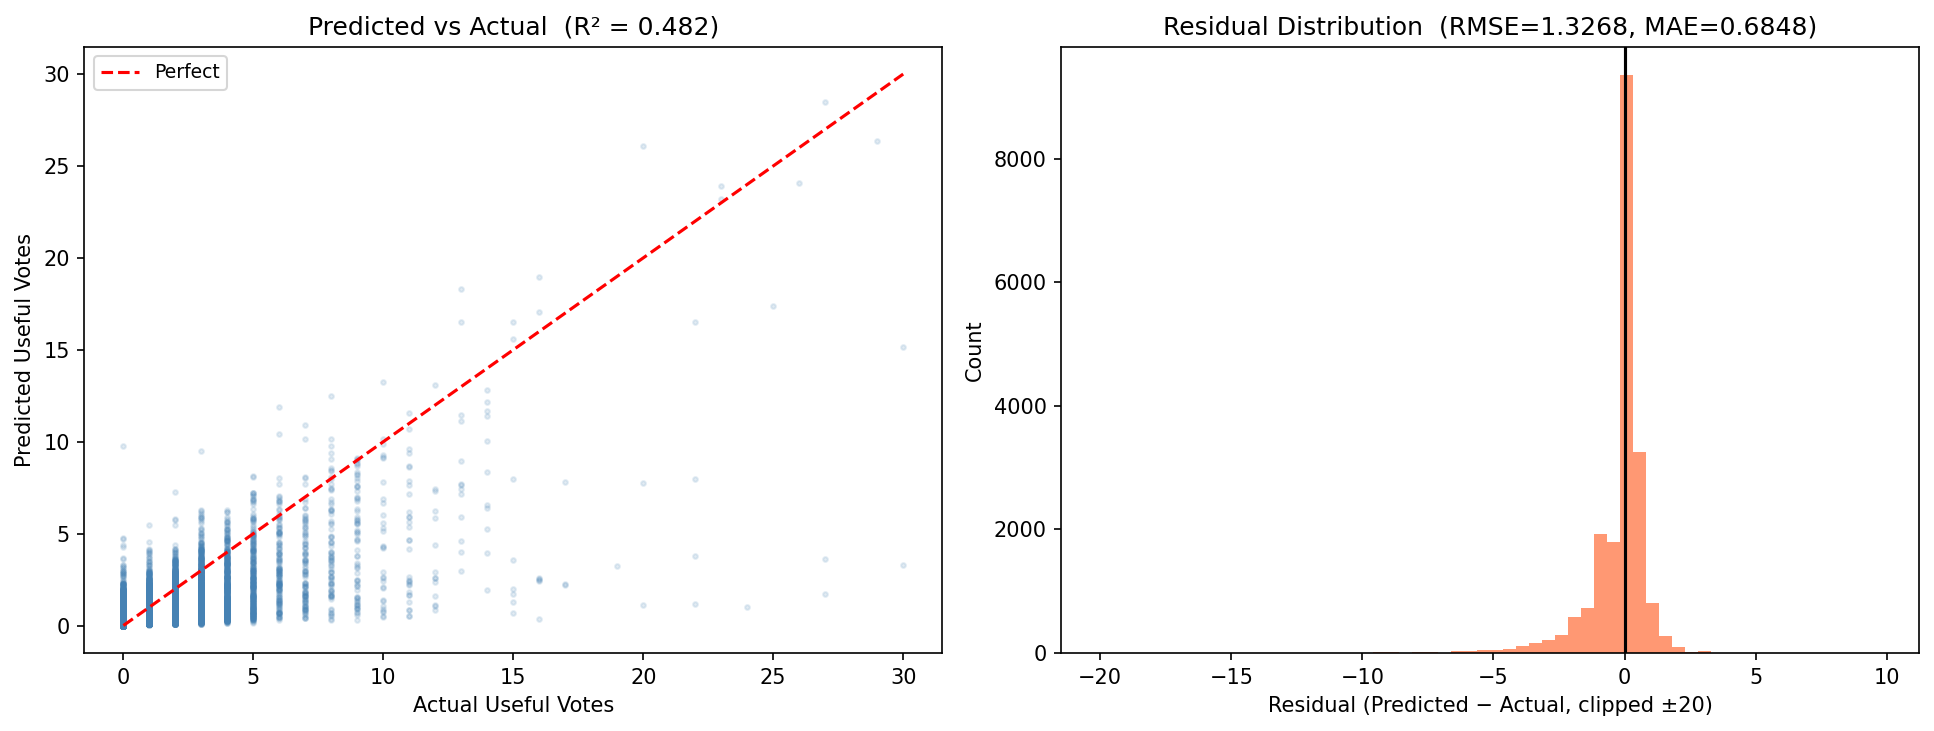
\includegraphics[width=\linewidth]{Report/PM_PredictedVsActual.png}
  \caption{Left: Predicted vs actual useful votes.
    Right: Residual distribution.}
\end{figure}

\begin{figure}[H]
  \centering
  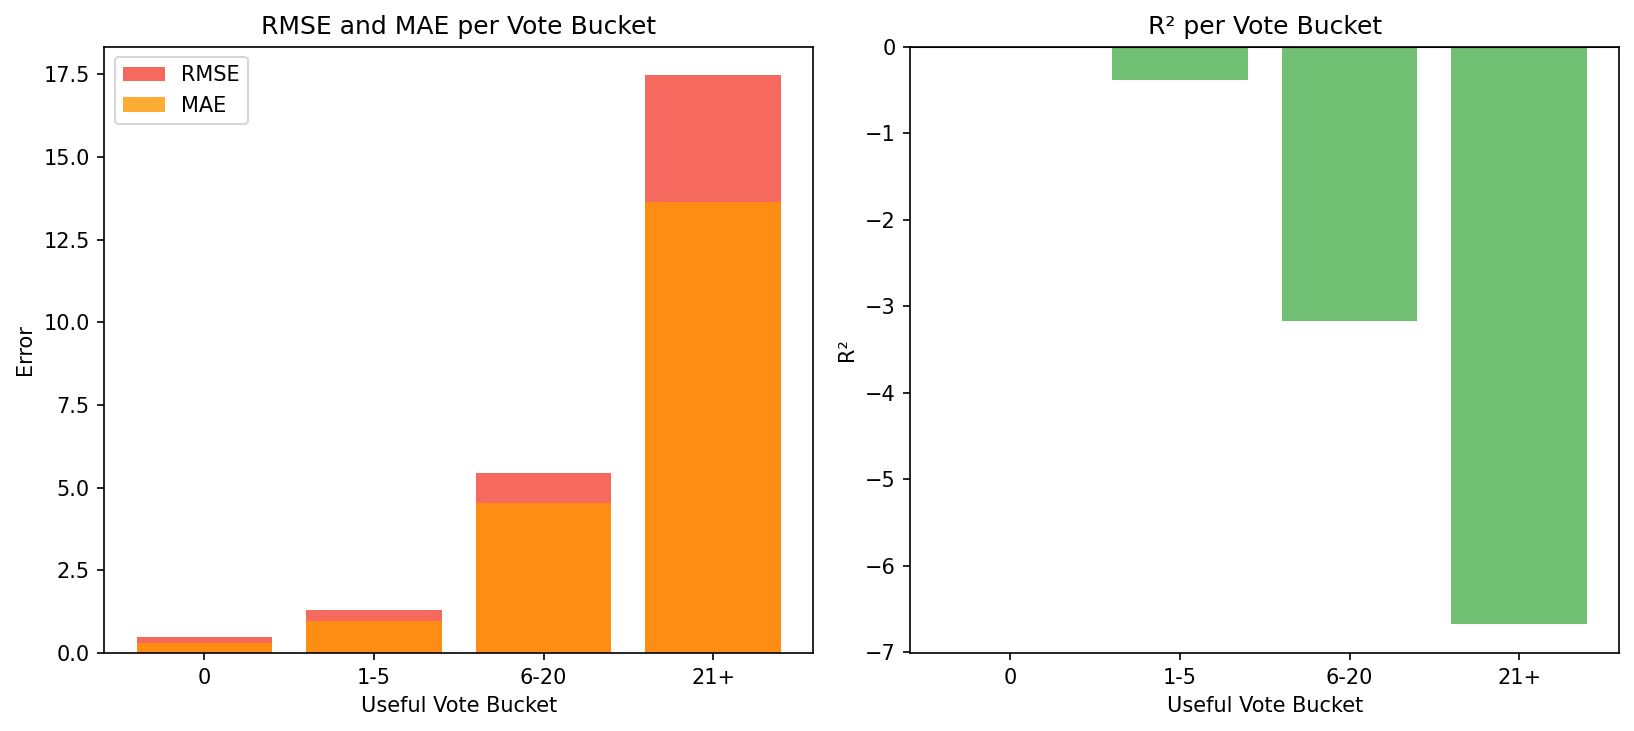
\includegraphics[width=0.75\linewidth]{Report/PM_BucketMetrics.png}
  \caption{RMSE, MAE, and R² broken down by useful-vote bucket.}
\end{figure}

\subsubsection*{Justification}

The $\log(1+y)$ transformation is essential because useful vote counts are
heavily right-skewed (most reviews receive 0 votes; a few receive hundreds).
Training directly on raw counts would bias the model toward predicting near-zero
values.  A Random Forest is appropriate here because it handles non-linear
interactions, is robust to outliers, and provides interpretable feature
importances without requiring feature scaling.  Stratified splitting ensures
the model is evaluated fairly across rare but important high-vote reviews.

% ─────────────────────────────────────────────────────────────────────────────
\subsection{Feature Importance and Discussion}

\begin{figure}[H]
  \centering
  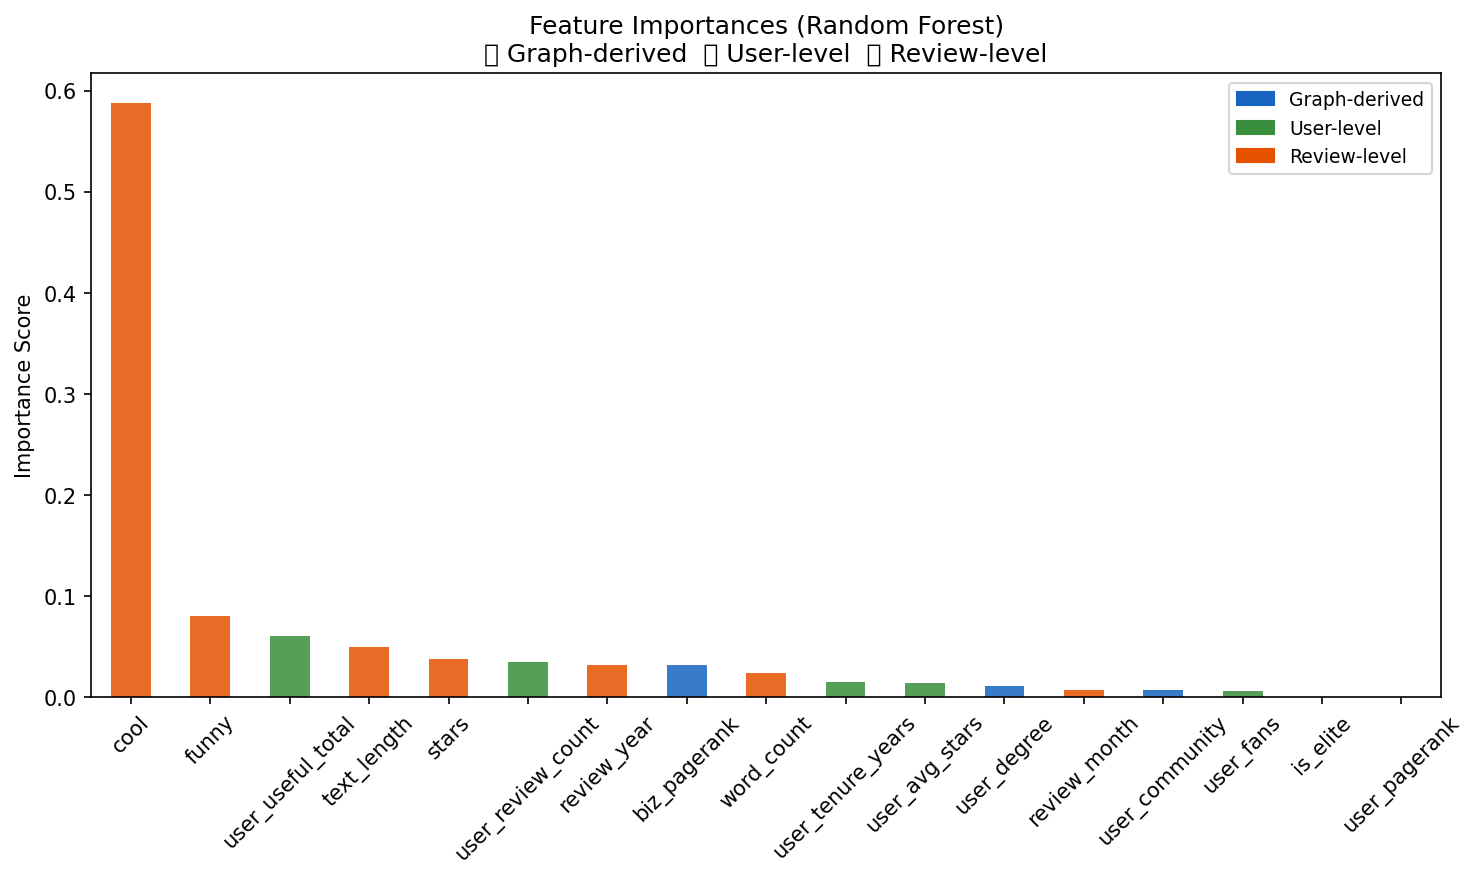
\includegraphics[width=0.85\linewidth]{Report/PM_FeatureImportances.png}
  \caption{Random Forest feature importances, grouped by feature type
    (blue = graph-derived, green = user-level, orange = review-level).}
\end{figure}

\textbf{Three most predictive features:}
\begin{enumerate}
  \item \textbf{cool} (importance = 0.588) —
    The ``cool'' vote is the single strongest predictor of usefulness: reviews
    that are perceived as engaging also tend to be perceived as informative,
    so both votes accumulate together, reflecting a unified community-approval
    signal.

  \item \textbf{funny} (importance = 0.080) —
    Entertaining reviews attract broader readership, which naturally increases
    their exposure and the probability of also receiving a useful vote; this
    spillover effect explains the second-largest predictor.

  \item \textbf{user\_useful\_total} (importance = 0.060) —
    A reviewer's cumulative useful-vote history is a strong credibility proxy:
    users who have consistently produced upvoted reviews continue to do so,
    reflecting a reputation feedback loop that drives future useful votes.
\end{enumerate}

\textbf{Limitations:}
\begin{enumerate}[noitemsep]
  \item \emph{Recency bias.}  The model is trained on historically accumulated useful votes, which reflects
    \emph{past} upvoting behaviour rather than intrinsic review quality.  Reviews written recently have had
    less time to accumulate votes, introducing temporal underestimation.  \texttt{review\_year} partially
    controls for this but does not fully remove the effect.
  \item \emph{Per-bucket generalisation failure.}  While the overall R$^2 = 0.48$ appears acceptable, the
    model performs \emph{worse than the bucket mean} for all non-zero vote buckets
    (R$^2 = -0.38$, $-3.17$, $-6.68$ for 1--5, 6--20, 21+ respectively).  The headline R$^2$ is inflated
    by the large proportion of zero-vote reviews (bucket 0), where the model predicts near-zero accurately.
    Predicting high useful-vote reviews — the most actionable targets — remains an open problem.
  \item \emph{Engagement-vote leakage.}  The top two predictors (\texttt{cool}, \texttt{funny}) are
    community-engagement votes that accumulate concurrently with useful votes.  Training on these features
    means the model partially learns ``reviews that received engagement also receive useful votes'' rather
    than learning what makes a review intrinsically useful.  In a deployment setting these signals would not
    be available at prediction time (before any votes arrive), limiting practical utility.
  \item \emph{Dead graph feature.}  \texttt{user\_pagerank} carries zero importance in both the link
    prediction and regression models.  Once \texttt{user\_review\_count}, \texttt{user\_avg\_stars}, and
    business-side PageRank are included, user-level PageRank adds no incremental signal.
\end{enumerate}

\textbf{Potential consequence of deployment:}
If such a model were used to rank reviews, it would systematically surface reviews
by highly connected, long-tenured reviewers and suppress reviews from new users —
even if those reviews are equally informative.  This creates a ``rich get richer''
dynamic that could entrench incumbent reviewers and discourage community growth.

\newpage
% ─────────────────────────────────────────────────────────────────────────────
\section*{AI Usage}
% ─────────────────────────────────────────────────────────────────────────────

AI assistance was used in the development of this assignment.
Conversation log: \url{https://gemini.google.com/u/1/app/a8a4f66f56882e2d?pageId=none}

\end{document}
